\PassOptionsToPackage{usenames,dvipsnames}{xcolor}

\documentclass[
12pt,
a4paper]{report}

\usepackage[usestackEOL]{stackengine}
\usepackage{url}
\usepackage{tocloft}
\usepackage{blindtext}

\usepackage{appendix}
\usepackage{todonotes}
\usepackage[cmex10]{amsmath}
%side by side tables with seperate captions: \RawFloats
\usepackage{floatrow}
%reference with "Table" infront of 3.1: \cref{}


\newcommand*{\appendixmore}{% S KOMA Doku S 339 
 \renewcommand*{\chapterformat}{ 
\appendixname~\thechapter\autodot\enskip} 
  \renewcommand*{\chaptermarkformat}{
\appendixname~\thechapter\autodot\enskip}} 

% Gruener Haken
\usepackage{rotating}
\newcommand*\rot{\rotatebox{270}}
\newcommand{\myGreen}[1]{{\color[RGB]{0,166,79}#1}}
\newcommand{\cmark}{\rot{\myGreen{$\checkmark$}}}%
\newcommand{\inmark}{\myGreen{$\checkmark$}}%

%\usepackage{showframe}% http://ctan.org/pkg/showframe
%\usepackage{etoolbox}% http://ctan.org/pkg/etoolbox

%\makeatletter
%\patchcmd{\@makechapterhead}{\vspace*{50\p@}}{\vspace*{10pt}}{}{}% Removes space above \chapter head
%\patchcmd{\@makeschapterhead}{\vspace*{50\p@}}{\vspace*{10pt}}{}{}% Removes space above \chapter* head
%\makeatother

\usepackage[left=3.5cm,right=2.5cm,top=2.5cm,bottom=2cm,includeheadfoot]{geometry}
\linespread{1.5}
\usepackage{lscape}

\usepackage{fancyhdr}

\pagestyle{fancy}

\fancypagestyle{plain}{
	\fancyhf{}
	
	\fancyfoot[R]{\footnotesize \thepage}
	\renewcommand{\headrulewidth}{0pt}
	\renewcommand{\footrulewidth}{.4pt}
}
\fancypagestyle{start}{
	\fancyhf{}
	
	%\renewcommand{\chaptermark}[1]{\markright{Abkürzungsverzeichnis}}
	\fancyhead[R]{\footnotesize \nouppercase{\rightmark}}
	\fancyfoot[R]{\footnotesize \thepage}
	\renewcommand{\headrulewidth}{.4pt}
	\renewcommand{\footrulewidth}{.4pt}
}
\fancypagestyle{middle}{
	\fancyhf{}

	\fancyhead[R]{\footnotesize \nouppercase{\leftmark}}
	\fancyfoot[R]{\footnotesize \thepage}
	\renewcommand{\headrulewidth}{.4pt}
	\renewcommand{\footrulewidth}{.4pt}
}
\fancypagestyle{end}{
	\fancyhf{}

	\fancyhead[R]{\footnotesize \nouppercase{\leftmark}}
	\fancyfoot[R]{\footnotesize \thepage}
	\renewcommand{\headrulewidth}{.4pt}
	\renewcommand{\footrulewidth}{.4pt}
}
\appto\frontmatter{\pagestyle{start}}
\appto\mainmatter{\pagestyle{middle}}
\appto\backmatter{\pagestyle{end}}

% hacks
%\usepackage{scrhack} 
%\usepackage{floatrow}



% Seitenrand für Korrektur
%\geometry{
%	left=2cm,
%  right=4.5cm
%}

%
% Textcodierung 
%
\usepackage[utf8]{inputenc}
\usepackage[T1]{fontenc}
\usepackage[full]{textcomp}
\usepackage{newtxtext,newtxmath,newtxtt}
\usepackage{courier}

\usepackage[babel]{microtype}
\usepackage{ellipsis}
\usepackage{setspace}

\usepackage{helvet}
\renewcommand{\familydefault}{\sfdefault}

% Nachfolgende Befehle schließen "Schusterjungen und Hurenkinder" aus.
\clubpenalty = 10000
\widowpenalty = 10000
\displaywidowpenalty = 10000

%
% Einstellungen für deutsche Texte
\usepackage[autostyle,babel,german=quotes,english=american]{csquotes}
\usepackage[USenglish,ngerman]{babel} 
\selectlanguage{ngerman}

%
% Schriftstile einstellen
%\setkomafont{sectioning}{\rmfamily\bfseries}
%\setkomafont{title}{\normalfont\rmfamily}
%\setkomafont{descriptionlabel}{\rmfamily}
%\setkomafont{caption}{\small\itshape} 
%\setkomafont{pageheadfoot}{\normalfont\normalcolor\footnotesize}
%\setcounter{secnumdepth}{3}
%\setcounter{tocdepth}{2}

\usepackage[tiny, compact]{titlesec}
\titleformat{\chapter}[display]
{\normalfont\normalsize\bfseries}{\chaptertitlename\ \thechapter}{20pt}{\normalsize}
\titlespacing*{\chapter}{0pt}{0pt}{40pt}


%
% Zitieren und Literaturverzeichnis mit biblatex
% Hinweis: UTF8 verlangt nach biber statt bibtex8
%\iffalse
\usepackage[%
 backend=biber,%
 style=authoryear,%
 bibstyle=alphabetic,%
 citestyle=authoryear,%
 natbib=false,%
 sorting=anyt,%
 sortcites=true,%
 hyperref=auto,%
 bibencoding=utf8,%
 sortlocale=de_DE,%
 maxcitenames=1,%
 maxbibnames=10,%
 minnames=1%
 %dashed=false%
]{biblatex}
%\fi

\DefineBibliographyStrings{ngerman}{ 
	andothers = {et\addabbrvspace al\adddot},
	andmore   = {et\addabbrvspace al\adddot},
}
%\DefineBibliographyStrings{ngerman}{andothers = {u.\,a.},}

\setcounter{biburllcpenalty}{7000}
\setcounter{biburlucpenalty}{8000}

% Quellenverzeichnisse
\addbibresource{bib/bib_articles.bib}
\addbibresource{bib/bib_online.bib}
\addbibresource{bib/bib_books.bib}

\setlength{\bibitemsep}{1em}



%
% Programmcode
\usepackage{listings}
\usepackage{diagbox,array,graphicx}
\usepackage[usenames,dvipsnames]{xcolor}

\definecolor{anti-flashwhite}{rgb}{0.95, 0.95, 0.96}
\definecolor{lightgray}{rgb}{.9,.9,.9}
\definecolor{darkgray}{rgb}{.4,.4,.4}
\definecolor{forestGreen}{RGB}{34,139,34}
\definecolor{orangeRed}{RGB}{255,69,0}
\definecolor{ghostwhite}{rgb}{0.97, 0.97, 1.0}
\definecolor{snow}{rgb}{1.0, 0.98, 0.98}
\definecolor{splashedwhite}{rgb}{1.0, 0.99, 1.0}
\definecolor{whitesmoke}{rgb}{0.96, 0.96, 0.96}

%%%%%%%%%%%%%%%%%%%%%%%%%%%%%%%%%%%%%%%%%%%%%%%%%%%%%%%%%%%%%%%%%%%%%%%%%%%%%%
%
% CODE LISTINGS
%
%%%%%%%%%%%%%%%%%%%%%%%%%%%%%%%%%%%%%%%%%%%%%%%%%%%%%%%%%%%%%%%%%%%%%%%%%%%%%%
% Define Language

%
% JAVA CODE
%

%JavaScript
\lstdefinelanguage{JavaScript}{
  keywords={typeof, new, true, false, catch, function, return, null, catch, switch, var, if, in, while, do, else, case, break},
  keywordstyle=\color{blue}\bfseries,
  ndkeywords={class, export, boolean, throw, implements, import, this},
  ndkeywordstyle=\color{darkgray}\bfseries,
  identifierstyle=\color{black},
  sensitive=false,
  comment=[l]{//},
  morecomment=[s]{/*}{*/},
  commentstyle=\color{purple}\ttfamily,
  stringstyle=\color{red}\ttfamily,
  morestring=[b]',
  morestring=[b]"
}

%%% PKCE GET
\lstdefinelanguage{PKCE}
{
	alsoletter={\\,/,\.,\-},
  % list of keywords
	  morekeywords={
		HTTP/1.1,
		GET,
		POST,
		Date,
		Location,
		Content-Type,
		Content-Length,
		Connection
  },
	morecomment=[s]{?code}{\~\~},
	morecomment=[s]{?code_challange}{j5U},
	morecomment=[s]{code_verifier}{GOQ},
	morecomment=[s]{?code_challenge_method}{\~\~},
	morecomment=[s]{\&code}{\~\~},
	morestring=[b]"',
	morecomment=[s]{\"access}{..\"},
	morecomment=[s]{\"refresh}{..\"},
	morecomment=[s]{\"Authorization}{..\"},
  sensitive=true, % keywords are not case-sensitive
	captionpos=b,
	basicstyle=\fontsize{8}{10}\selectfont\ttfamily,
	showstringspaces=false,
	numbers=left,
	numberstyle=\tiny,
	tabsize=2,
	numbersep=3pt,
	extendedchars=true,
	xleftmargin=2em,
	lineskip=1pt,
	breaklines,
	%Coloring
	backgroundcolor=\color{splashedwhite},
	identifierstyle=\color{black}\ttfamily,
	stringstyle=\color{black}\ttfamily,
	commentstyle=\color{blue}\ttfamily
}
%%%

\lstdefinelanguage{POST}
{
  % list of keywords
  morekeywords={
		grant_type,
		code,
		client_assertion,
		client_assertion_type,
		code_verifier,
		client_id
  },
  sensitive=false, % keywords are not case-sensitive
  morestring=[b]", % defines that strings are enclosed in double quotes
	morestring=[b]:,
	morestring=[b]=,
	captionpos=b,
	basicstyle=\fontsize{8}{10}\selectfont\ttfamily,
	showstringspaces=false,
	numbers=left,
	numberstyle=\tiny,
	tabsize=2,
	numbersep=3pt,
	extendedchars=true,
	xleftmargin=2em,
	lineskip=1pt,
	breaklines,
	%Coloring
	backgroundcolor=\color{splashedwhite},
	identifierstyle=\color{blue}\ttfamily,
	stringstyle=\color{black}\ttfamily,
	commentstyle=\color{forestGreen}\ttfamily
}
%%%%%%%%%%%%%%%%%%%%%%%%%%%%%%%%%%%%%%%%%%%%%%%%%%%%%%%%%%%%%%%%%%%%%%%%%%%%%%
\lstdefinelanguage{HTTP32}
{
	alsoletter=-,
  % list of keywords
	  morekeywords={
		POST,
		Host,
		SAMLart,
		RelayState,
		User-Agent,
		Content-Type,
		Content-Length,
		Parameter
  },
	morecomment=[s]{AAQ}{An},	
  sensitive=false, % keywords are not case-sensitive
	captionpos=b,
	basicstyle=\fontsize{8}{10}\selectfont\ttfamily,
	showstringspaces=false,
	numbers=left,
	numberstyle=\tiny,
	tabsize=2,
	numbersep=3pt,
	extendedchars=true,
	xleftmargin=2em,
	lineskip=1pt,
	breaklines,
	%Coloring
	backgroundcolor=\color{splashedwhite},
	identifierstyle=\color{black}\ttfamily,
	stringstyle=\color{black}\ttfamily,
	commentstyle=\color{blue}\ttfamily
}
%%%%%%%%%%%%%%%%%%%%%%%%%%%%%%%%%%%%%%%%%%%%%%%%%%%%%%%%%%%%%%%%%%%%%%%%%%%%%%
\lstdefinelanguage{HTTP31}
{
	alsoletter=-,
  % list of keywords
	  morekeywords={
		POST,
		Host,
		SAMLart,
		RelayState,
		User-Agent,
		Content-Type,
		Content-Length,
		Parameter
  },
	morecomment=[s]{PHN}{dD4},	
  sensitive=false, % keywords are not case-sensitive
	captionpos=b,
	basicstyle=\fontsize{8}{10}\selectfont\ttfamily,
	showstringspaces=false,
	numbers=left,
	numberstyle=\tiny,
	tabsize=2,
	numbersep=3pt,
	extendedchars=true,
	xleftmargin=2em,
	lineskip=1pt,
	breaklines,
	%Coloring
	backgroundcolor=\color{splashedwhite},
	identifierstyle=\color{black}\ttfamily,
	stringstyle=\color{black}\ttfamily,
	commentstyle=\color{blue}\ttfamily
}
%%%%%%%%%%%%%%%%%%%%%%%%%%%%%%%%%%%%%%%%%%%%%%%%%%%%%%%%%%%%%%%%%%%%%%%%%%%%%%
\lstdefinelanguage{HTTPget302}
{
	alsoletter={\\,/,\.,\-},
  % list of keywords
	  morekeywords={
		HTTP/1.1,
		Date,
		Location,
		Content-Type
  },
	morecomment=[s]{BLD}{bB6},	
	morecomment=[s]{PHNhu}{VzdD4},
  sensitive=true, % keywords are not case-sensitive
	captionpos=b,
	basicstyle=\fontsize{8}{10}\selectfont\ttfamily,
	showstringspaces=false,
	numbers=left,
	numberstyle=\tiny,
	tabsize=2,
	numbersep=3pt,
	extendedchars=true,
	xleftmargin=2em,
	lineskip=1pt,
	breaklines,
	%Coloring
	backgroundcolor=\color{splashedwhite},
	identifierstyle=\color{black}\ttfamily,
	stringstyle=\color{black}\ttfamily,
	commentstyle=\color{blue}\ttfamily
}
%%%%%%%%%%%%%%%%%%%%%%%%%%%%%%%%%%%%%%%%%%%%%%%%%%%%%%%%%%%%%%%%%%%%%%%%%%%%%%
\lstdefinelanguage{302OAuth}
{
	alsoletter={\\,/,\.,\-},
  % list of keywords
	  morekeywords={
		HTTP/1.1,
		GET,
		POST,
		Date,
		Location,
		Content-Type,
		Content-Length,
		Connection
  },
	morecomment=[s]{https}{callback},
	morecomment=[s]{?code}{\~\~},
	morecomment=[s]{\&code}{\~\~},
	morestring=[b]"',
	morecomment=[s]{\"access}{..\"},
	morecomment=[s]{\"refresh}{..\"},
	morecomment=[s]{\"Authorization}{..\"},
  sensitive=true, % keywords are not case-sensitive
	captionpos=b,
	basicstyle=\fontsize{8}{10}\selectfont\ttfamily,
	showstringspaces=false,
	numbers=left,
	numberstyle=\tiny,
	tabsize=2,
	numbersep=3pt,
	extendedchars=true,
	xleftmargin=2em,
	lineskip=1pt,
	breaklines,
	%Coloring
	backgroundcolor=\color{splashedwhite},
	identifierstyle=\color{black}\ttfamily,
	stringstyle=\color{black}\ttfamily,
	commentstyle=\color{blue}\ttfamily
}

%%%%
\lstdefinelanguage{302OAuthGET}
{
	alsoletter={\\,/,\.,\-},
  % list of keywords
	  morekeywords={
		HTTP/1.1,
		GET,
		Host,
		User-Agent,
		POST,
		Date,
		Location,
		Content-Type,
		Content-Length,
		Connection
  },
	morecomment=[s]{Authorization}{..},
	morecomment=[s][\color{red}]{<!--}{-->},
	morecomment=[s]{\&access}{...},
  sensitive=true, % keywords are not case-sensitive
	captionpos=b,
	basicstyle=\fontsize{8}{10}\selectfont\ttfamily,
	showstringspaces=false,
	numbers=left,
	numberstyle=\tiny,
	tabsize=2,
	numbersep=3pt,
	extendedchars=true,
	xleftmargin=2em,
	lineskip=1pt,
	breaklines,
	%Coloring
	backgroundcolor=\color{splashedwhite},
	identifierstyle=\color{black}\ttfamily,
	stringstyle=\color{black}\ttfamily,
	commentstyle=\color{blue}\ttfamily
}

\lstdefinelanguage{bpel}{
morekeywords={name,linkName,isolated,parallel,partnerLink,operation,portType,inputVariable,createInstance,
variable,element,location,importType,partnerLinkType,myRole,messageType,properties,level,outputVariable,
xmlns,version,encoding}
}
\lstdefinelanguage{xaml}{
morekeywords={TypeArguments,Name,Default,DisplayName,OperationName,ServiceContractName,Key,AddressUri,
CanCreateInstance, LogName, Message, MessageNumber, Expression,CorrelationHandle,Request}
}

\lstdefinestyle{workflowStyle}{
	language=XML,
	alsolanguage=bpel,
	alsolanguage=xaml,
	captionpos=b,
%Formatting
%basicstyle=\scriptsize,
	basicstyle=\fontsize{8}{10}\selectfont\ttfamily,
	sensitive=true,
	showstringspaces=false,
	numbers=left,
	numberstyle=\tiny,
	tabsize=2,
	numbersep=3pt,
	extendedchars=true,
	xleftmargin=2em,
	lineskip=1pt,
	breaklines,
	%Coloring
	backgroundcolor=\color{splashedwhite},
	morekeywords={BooleanExpression},
	alsoletter={:,,/,?},
	morestring=[b]{"},
	morecomment=[s]{&lt;!--}{--&gt;},keywordstyle=\color{forestGreen},
	identifierstyle=\color{blue}\ttfamily,
	stringstyle=\color{orangeRed}\ttfamily,
	commentstyle=\color{forestGreen}\ttfamily
}

\lstdefinelanguage{XML}
{
  morestring=[s][\color{mauve}]{"}{"},
  morestring=[s][\color{black}]{>}{<},
  morecomment=[s]{<?}{?>},
  morecomment=[s][\color{forestGreen}]{<!--}{-->},
  stringstyle=\color{black},
  identifierstyle=\color{lightblue},
  keywordstyle=\color{red},
  morekeywords={xmlns,xsi,noNamespaceSchemaLocation,type,id,x,y,source,target,version,tool,transRef,roleRef,objective,eventually}% list your attributes here
}

% 
% PDF Erstellung steuern und Links aktivieren
\usepackage{pdfpages}
\usepackage[hidelinks]{hyperref} 
% PDF \usepackage[hidelinks]{hyperref} 
\urlstyle{rm}
\usepackage{color}
\definecolor{darkblue}{rgb}{0,0,.5}
\hypersetup{%
   pdftitle={Name, Titel},
   pdfauthor={Vorname Name},
   pdfstartview=FitH,
   pdfpagelayout=OneColumn,
   naturalnames=false,%
   colorlinks=false,%
	 linkcolor=black,%
	 % Farbige Links für PDF
	 %colorlinks=true,
	 %linkcolor=blue,%
   breaklinks=true,%
   citecolor=black,%
   filecolor=black,%
   urlcolor=black}
   
%
% Semantische Textauszeichnung
%
\newcommand{\meta}[1]{\texttt{#1}}
\newcommand{\fat}[1]{\textbf{#1}} 
\newcommand{\product}[1]{\textsc{#1}} 

%
% Figures and graphics
% 
\usepackage{graphicx}
\graphicspath{/img}
\usepackage{booktabs}
\usepackage{tabularx}
\usepackage{multirow}
\newcolumntype{L}[1]{>{\raggedright\arraybackslash}p{#1}}
\newcolumntype{C}[1]{>{\centering\arraybackslash}p{#1}}
\newcolumntype{R}[1]{>{\raggedleft\arraybackslash}p{#1}}

% 
% helpful packages
%
\usepackage{enumerate}
\usepackage{varioref}
\usepackage{cleveref}

\newcommand{\verylongpage}{\enlargethispage{2\baselineskip}}
\usepackage{blindtext}
%\usepackage[ngerman=ngerman-x-latest]{hyphsubst}
%\hyphenation{%
%Wirt-schafts-in-for-ma-tik
%Ge-schäfts-pro-zess-mo-dell
%Ge-schäfts-prozess-modell-ier-ung
%}

%
% Useful abbreviations
\usepackage{xspace} 
\newcommand{\msc}{M.\,Sc.\@\xspace}
\newcommand{\MSc}{M.\,Sc.\@\xspace}
\newcommand{\bsc}{B.\,Sc.\@\xspace}
\newcommand{\BSc}{B.\,Sc.\@\xspace}
\newcommand{\dH}{d.\,h.\@\xspace}

\newenvironment{myquote}{\begin{quote} \small}{\end{quote}}

%\renewcommand\uppertitleback[1]{\thispagestyle{empty}#1\vfill}
%\renewcommand\lowertitleback[1]{#1}

%%%%%%%%%%%%%%%%%%%%%%%%%%%%%%%%%%%%%%%%%%%%%%%%%%%%%%%%%%%%%%%%%%%%%%%%%%%%%%%
\usepackage{color}
\definecolor{shadecolor}{gray}{.70}
%%%%%%%%%%%%%%%%%%%%%%%%%%%%%%%%%%%%%%%%%%%%%%%%%%%%%%%%%%%%%%%%%%%%%%%%%%%%%%%

\usepackage[framemethod=TikZ]{mdframed}
\usepackage{xcolor}
\usepackage[all]{hypcap}
%\usepackage{longtable}

\definecolor{light-gray}{gray}{0.85}

\newmdenv[%
backgroundcolor=light-gray,
linecolor=light-gray,
skipabove=1\baselineskip,
skipbelow=1\baselineskip,
]{shaded}

\newmdenv[%
%backgroundcolor=light-gray,
linecolor=black,
outerlinewidth=1pt,
%roundcorner=2mm,
skipabove=1\baselineskip,
skipbelow=1\baselineskip,
]{syntax}

\usepackage{todonotes}
\usepackage{tabu}
\usepackage{longtable}
\usepackage{acro}
\usepackage{mfirstuc}% provides \makefirstuc
\usepackage{tocloft}
\usepackage[automake]{glossaries}
\renewcommand{\glossarypreamble}{\glsfindwidesttoplevelname[\acronymtype] \setlength{\parskip}{0pt}}

\renewcommand\cftloftitlefont{\normalfont \bf}
\renewcommand\cftlottitlefont{\normalfont \bf}
\renewcommand\cfttoctitlefont{\normalfont \bf}

\setlength{\cftbeforetoctitleskip}{41pt} % TOC: Table of Contents
\setlength{\cftbeforeloftitleskip}{41pt} % LOF: Listing of Figures
\setlength{\cftbeforelottitleskip}{41pt} % LOT: Listing of Tables
\setlength{\cfttabindent}{0em}



\acsetup{
	first-style=short,
	pages/display=first,
	list/template=lof,
	list/heading=chapter,
	list/name=Abkürzungsverzeichnis
}
\DeclareAcronym{lda}{
	short = LDA ,
	long  = Latent Dirichlet Allocation
}
\DeclareAcronym{dlda}{
	short = DLDA ,
	long  = Dynamic Latent Dirichlet Allocation
}
\DeclareAcronym{hlda}{
	short = HLDA ,
	long  = Hierarchic Latent Dirichlet Allocation
}
\DeclareAcronym{crp}{
	short = CRP ,
	long  = Chinese Restaurant Process
}
\DeclareAcronym{tf-idf}{
	short = tf-idf ,
	long  = Term Frequency-Inverse Document Frequency
}
\DeclareAcronym{cvt}{
	short = CVT ,
	long  = Continiuously Variable Transmission
}
\DeclareAcronym{bow}{
	short = BoW ,
	long  = Bag-of-Words
}
\DeclareAcronym{tdm}{
	short = TDM ,
	long  = Term-Dokument Matrix
}
\DeclareAcronym{ipmi}{
	short = IPMI ,
	long  =  Institute of Project Management and Innovation
}
\DeclareAcronym{gm}{
	short = GM ,
	long  =  General Motors,
	tag = abbrev
}

\makeglossaries
\renewcommand*\glspostdescription{\dotfill}


\newacronym{lda}{LDA}{Latent Dirichlet Allocation}
\newacronym{hlda}{HLDA}{Hierarchical Latent Dirichlet Allocation}
\newacronym{dlda}{DLDA}{Dynamic Latent Dirichlet Allocation}
\newacronym{evt}{EVT}{Electrically Variable Transmission}
\newacronym{cvt}{CVT}{Continuously Variable Transmission}
\newacronym{pyLDAvis}{pyLDAvis}{Python LDA Visualization}

\begin{document}

%%%%%%%%%%%%%%%%%%%%%%%%%%%%%%%%%%%%%%%%%%%%%%%%%%%%%%%%%%%%%%
%%%%%%%%%%%%%%%%%%%%%%%%%%%%%%%%%%%%%%%%%%%%%%%%%%%%%%%%%%%%%%
%
% TITELSEITE 1
%
%%%%%%%%%%%%%%%%%%%%%%%%%%%%%%%%%%%%%%%%%%%%%%%%%%%%%%%%%%%%%%
\thispagestyle{empty}
\pagenumbering{Alph}
\begin{titlepage}
\thispagestyle{empty}
  \begin{center}
	
	% Unilogo
  
\includegraphics[scale=0.2]{img/Universitaet_Bremen}\\ \vspace{0.0cm}

	% Fachbereich
	{\Large{\scshape Fachbereich 3}}\\
  {\Large{\scshape Fakultät für Mathematik und Informatik}}\\[2.5cm]
	
	% Thesis-Thema
	{\LARGE Topic Modeling basierte Analyse eines Patentdatensatzes von General Motors}
  \vspace{2.0cm}
	  
	% Bachelor- oder Master-Thesis und Studiengang
  Abschlussarbeit im Studiengang\\
	Bachelor of Science Wirtschaftsinformatik\\
	der Universität Bremen\\[3cm]

	% Studenteninformationen
  \begin{tabular}[c]{lll}
		Name,Vorname: & Tietjen, Hauke\\
		Matrikelnummer: & 4224296\\
		Datum: & XX.XX.XXX \\
		Studiengang: & Wirtschaftsinformatik, Bachelor of Science\\
		Eingereicht bei: & Prof. Dr. Martin G. Möhrle (Universität Bremen)\\
		 & Prof. Dr. Jutta Günther (Universität Bremen)
	\end{tabular}
  \end{center}
\end{titlepage}
\newpage
\newpage
%%%%%%%%%%%%%%%%%%%%%%%%%%%%%%%%%%%%%%%%%%%%%%%%%%%%%%%%%%%%%%

%%%%%%%%%%%%%%%%%%%%%%%%%%%%%%%%%%%%%%%%%%%%%%%%%%%%%%%%%%%%%%
%
% Leere Seite 2
%
%%%%%%%%%%%%%%%%%%%%%%%%%%%%%%%%%%%%%%%%%%%%%%%%%%%%%%%%%%%%%%
%\mbox{} 
%\thispagestyle{empty}
%\newpage



\frontmatter
\pagenumbering{Roman}
\tableofcontents

\clearpage \newpage

%\cftsetindents{entry}{indent}{numwidth}
%\setlength\cftsecnumwidth{5em}

\phantomsection
\addcontentsline{toc}{chapter}{Abkürzungsverzeichnis}

%\setlength{\cftsecindent}{10em}
%\cftsetindents{figure}{0em}{3.5em}
%\cftsetindents{table}{0em}{3.5em}
%\printacronyms
%
%\glsaddall
\printglossary[title=Abkürzungsverzeichnis,style=alttree]
\clearpage
\newpage
\phantomsection
\addcontentsline{toc}{chapter}{Abbildungsverzeichnis}
\listoffigures
\clearpage \newpage
\phantomsection
\addcontentsline{toc}{chapter}{Tabellenverzeichnis}
\listoftables
\clearpage \newpage
%%%%%%%%%%%%%%%%%%%%%%%%%%%%%%%%%%%%%%%%%%%%%%%%%%%%%%%%%%%%%%%%%%%%%%%%%%%%%%%%%%

% Setup für Fußnoten
%\setlength{\skip\footins}{2em}		% Fußnoten um 2em nach unten versetzt

%%%%%%%%%%%%%%%%%%%%%%%%%%% INHALT %%%%%%%%%%%%%%%%%%%%%%%%%%%%%%%%%%%%%%%%%%%%
\mainmatter
\pagenumbering{arabic}
%\setcounter{page}{1}
% Für Korrektur
%\doublespacing

\lstset{language=C}

%%%%%%%%%%%%%%%%%%%%%%%%%%%%%%%%%%%%%%%%%%%%%%%%%%%%%%%%%%%%%%%%
%
% Kapitel: EINLEITUNG
%
%%%%%%%%%%%%%%%%%%%%%%%%%%%%%%%%%%%%%%%%%%%%%%%%%%%%%%%%%%%%%%%%

\chapter{Einleitung}
\section{Thema}
In dieser Bachelorarbeit geht es darum, die relevantesten Themen in einem großen Patentdatensatz von \gls{gm} zu finden. Dazu werden generativen Wahrscheinlichkeitsmethoden verwendet werden. Diese Themen sollen benannt und graphisch dargestellt werden. Außerdem gilt es herauszufinden welche Themengruppen vorhanden sind und welche Patente zu einem oder mehreren Themen gehören. Außerdem soll der Trend der Themen über die Jahre untersucht werden.

% 2. Problemstellung
\section{Motivation und Forschungsfragen}
Uns standen noch nie so viele Informationen zur Verfügung wie heute und jeden Tag kommen neue hinzu. Wir durchsuchen schriftliche Informationen nach Stichwörtern, mit der Hilfe von Suchmaschinen. So lassen sich zu einem Thema schnell mehrere Texte finden.

Man beschreibt ein Thema aus Stichwörtern und sucht Texte, welche diese enthalten. Wenn man diese Suche umkehrt, funktioniert sie nicht mehr. Man hat einen Datensatz aus Texten und möchte alle darin enthaltenen Themen herausfinden. Intuitiv denkt man hier an den Titel aber der reicht nicht aus, um alle Themen eines Textes zu beschreiben. Allein der Titel dieser Arbeit verschweigt das Thema des Preprocessings. Manche Texte haben Schlagworte aber dabei verlässt man sich auf den Autor, diese Richtigen zu wählen und sie werden nicht nach Relevanz gewichtet. Außerdem könnte man, mit dem Wissen über die Trends der Patentthemen, Vermutungen über die Patentthemen der Zukunft anstellen.

Topic Modeling ist besonders interessant, weil mit relativ geringem Aufwand große Mengen an Dokumenten untersucht werden können. Dadurch könnten, speziell in diesem Fall, die Konkurrenten von General Motors herausfinden, worum es in den Datensatz geht und in welche Richtung sich die Themen der Patente in Zukunft entwickeln könnten. Wodurch sie General Motors bei der Anmeldung neuer Patenten zuvorkommen und Lizenzgebühren verlangen könnten.

Die Forschungsfragen dieser Arbeit sind:
\begin{itemize}
	\item Welche relevanten Themen befinden sich in dem Datensatz?
	\item Wie sind diese Themen zu benennen?
	\item Welchen Gruppen gehören diese Themen an?
	\item Welche Trends haben diese Themen? 
\end{itemize}

% 3. Zielsetzung
\section{Methodisches Vorgehen}
Um die versteckten Themen zu finden, werden generative Wahrscheinlichkeitsmethoden benutzt. Eine Methode ist die Latent Dirichlet Allocation \parencite[vgl.][]{Blei03latentdirichlet}. Zuerst wird eine bestimmte Zahl an Themen festgelegt. Wörter die häufig gemeinsam vorkommen werden einem gemeinsamen Thema zugeordnet. Nachdem alle Wörter mindestens einem Thema zugeordnet wurden, wird der Vorgang für eine höhere Zahl an Themen wiederholt bis man genug Modelle hat, um sie zu vergleichen. Aus den Modellen wird das mit der höchsten Kohärenz ausgewählt \parencite[vgl.][]{TopicCoherence}.

Die wahrscheinlichsten Wörter eines Themas könnten lauten Ventil, Hydraulik und Flüssigkeit. Dieses Thema kann dann wiederum Texten zugeordnet werden. Mit dieser Methode lassen sich die Themen eines Datensatzes von tausenden Dokumenten viel schneller benennen, als es einem Menschen durch normales Lesen möglich wäre. Dazu wird das Online Latent Dirichlet Allocation Verfahren angewandt. \parencite[vgl.][]{Hoffman10onlinelearning} Als Kohärenzmaß wird C\_umass verwendet \parencite[vgl.][]{TopicCoherence}.

Der Patentdatensatz von General Motors umfasst 1410 Patente für verschiedene Getriebearten und ist ausreichend groß, um Topic Modeling zu betreiben. Um diese Untersuchungen zu realisieren, wird die Programmiersprache Python verwenden. Mit Hilfe der Programmbibliothek gensim werden die Modelle erstellen und die Kohärenzen ausgewertet \parencite[vgl.][]{rehurek_lrec}. Die Ergebnisse werden mit \gls{pyLDAvis} untersucht, um in einem qualitativen Verfahren Gruppen zu bilden und Themen zu benennen \parencite[vgl.][]{sievert2014ldavis}. Die Gruppen sollen mit \gls{hlda} bestätigt werden \parencite[vgl.][]{griffiths2004hierarchical}.

Des weiteren soll mit dem \gls{dlda} Verfahren herausgefunden werden wie sich die Themen des Datensatzes, entlang der zeitlichen Anmeldedaten der Patente, verändert haben \parencite[vgl.][]{dynamicLDA}. Eine Vorhersage wäre für ein konkurrierendes Unternehmen hilfreich, um Patente vor General Motors anzumelden und Lizenzgebühren verlangen zu können.
















\chapter{Begriffliche Grundlagen}

\section{Latent Dirichlet Allocation}
\todo[inline]{Herr Möhrle hat gesagt bei längeren Zitaten, Verweis nach dem ersten Satz}
\todo[inline]{Bei Erstverwendung einer Abkürzung (ABK) in Klammern?}
Die \acrfull{lda} ist ein generatives Wahrscheinlichkeitsmodell für Textdokumente. \parencite[vgl.][S. 996]{Blei03latentdirichlet} Dokumente werden als zufällige Mischverteilungen über latente Themen dargestellt, wobei jedes Thema eine Wahrscheinlichkeitsverteilung über Worte ist. 

Vereinfacht gesagt werden alle Dokumente mit einer Wahrscheinlichkeit zu vorher unbekannten Themen zugeordnet. Die Themen werden also durch den Algorithmus gefunden. Ein Thema besteht aus der Menge aller in den Dokumenten vorkommenden Wörtern und ihrer Wahrscheinlichkeit das sie zu diesem Thema gehören.
\todo{zitat finden}
Die Reihenfolge der Dokumente ist nicht relevant. Auch die Reihenfolge der Wörter in den Dokumenten wird nicht beachtet, sondern nur die Häufigkeit, es gilt das \acl{bow} Modell. \parencite[vgl.][S. 155-156]{harris1954distributional} Die Anzahl der latenten Themen muss vorher gegeben sein.
\todo{beispiel geben zu LDA}
Um die Anzahl an versteckten Themen zu approximieren werden alle \ac{lda} Modelle mit den Themenanzahlen von 1 bis 100 erstellt. Diese Modelle werden anhand ihrer Kohärenz innerhalb der Themen und anhand ihrer Distanz zwischen den Themen verglichen. Mithilfe dieser Daten sucht man ein Modell aus, das eine möglichst geringe Themenanzahl, hohe Kohärenz und hohe Distanz aufweist. Die Themenanzahl sollte möglichst gering sein, weil es aufwändig ist diese Themen zu interpretieren und die Distanz bei zu hoher Themenzahl sinkt.

\begin{figure}[htpb]
	\centering
	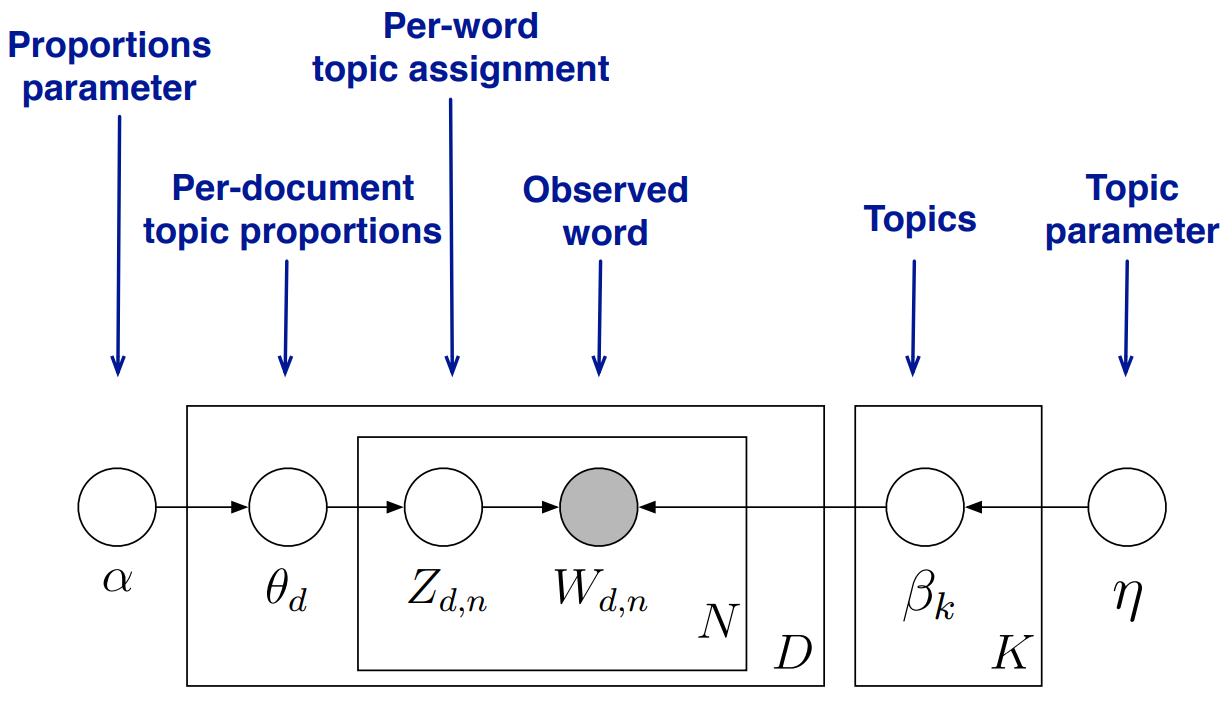
\includegraphics[width=\textwidth,height=8cm,keepaspectratio=true]{lda.png}
	\caption{
		LDA als graphisches Modell, von \parencite[vgl.][S. 23]{ProbabilisticTopicModels}
	}
	\label{fig:LDA Modell}
\end{figure}


$\mathcal{W}$ ist das Wort aus $\mathcal{N}$ Wörtern eines Dokuments i. Dieses Dokument i ist eines aus allen Dokumenten $\mathcal{M}$. Alle folgenden Parameter sind latent. $\mathcal{Z}$ ist das Thema für das Wort j aus besagtem Dokument i. Jedem Wort wird ein Thema zugeordnet. Wodurch jedes Dokument eine Mischung aus allen Themen ist. Die Verteilung der Themen für Dokument i ist $\theta$. Die Hyperparameter $\alpha$ und $\beta$ der \acl{lda}. $\alpha$ bestimmt die Dokument-Themen Verteilung und die Wort-Themen Verteilung. Ein hoher $\alpha$ Wert erhöht die Wahrscheinlichkeit dafür das einem Dokument mehr Themen zugeordnet werden. Ein niedriger $\alpha$ Wert verringert die Wahrscheinlichkeit das einem Dokument mehrere Themen zugeordnet werden. Ein hoher $\beta$ Wert erhöht die Wahrscheinlichkeit das einem Thema mehr Wörter zugeordnet werden. Ein niedriger $\beta$ Wert erhöht die Wahrscheinlichkeit das einem Thema weniger Wörter zugeordnet werden. Vereinfacht gesagt lässt ein großer $\alpha$ Wert die Dokumente ähnlicher aussehen und ein hoher $\beta$ Wert lässt die Themen ähnlicher aussehen. Mit diesem Algorithmus lässt sich ein Model erstellen, das jedes Wort mit Wahrscheinlichkeit zu jedem Thema zuordnet.

\begin{figure}[htpb]
	\centering
	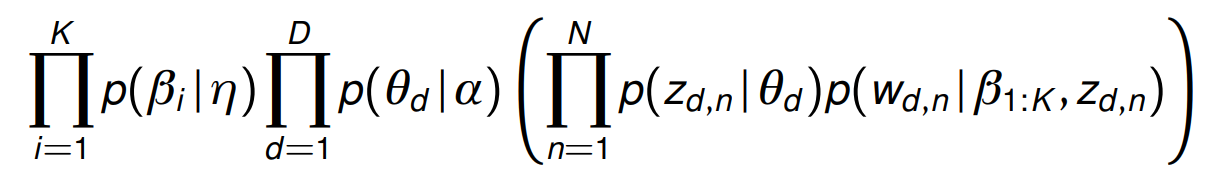
\includegraphics[width=\textwidth,height=3cm,keepaspectratio=true]{ldaDocLikelyhood.png}
	\caption{
		LDA als graphisches Modell, von \parencite[vgl.][S. 25]{ProbabilisticTopicModels}
	}
	\label{fig:LDA Formel}
\end{figure}


Dies ist die Wahrscheinlichkeit ein Dokument zu generieren, mit den Einstellungen des \ac{lda} Modells. Die Wahrscheinlichkeit ist gering aber je höher sie ist desto besser ist das Modell. Die vier Komponenten der Formel sind die Einstellungen des \ac{lda} Modells als Faktoren. Diese ergeben wiederum eigene Wahrscheinlichkeiten. Der Erste Faktor ist eine Dirichletverteilung von Dokumenten zu Themen. Eine Dirichletverteilung kann man sich als n-Simplex vorstellen, mit n gleich der Anzahl von Themen. Jedes Dokument hat eine Wahrscheinlichkeit für die Zugehörigkeit zu jedem Thema. Die Dirichletverteilung ist also eine Verteilung von Verteilungen. Der zweite Faktor ist eine Dirichletverteilung von Themen zu Wörtern und verhält sich analog zur ersten.

Der dritte Faktor ist eine Multinomialverteilung des ersten Faktors. Eine Multinomialverteilung ist wie eine Urne mit mehreren verschiedenen Themen, die mit Wahrscheinlichkeiten gezogen werden können. Diese zweite Multinomialverteilung ist also eine von Themen. Der Vierte Faktor ist eine Multinomialverteilung des zweiten Faktors mit Worten. Diese verhält sich analog zur ersten.

Kombiniert man diese Multinomialverteilungen miteinander, indem man immer ein Thema aus der ersten zieht und zu dem Thema passend ein Wort aus der zweiten, generiert man ein neues Dokument. Dies wird wiederholt bis gleich viele Dokumente generiert wurden wie verarbeitet wurden. Die Wahrscheinlichkeit das man mit dieser Methode die gleichen Dokumente erzeugt ist wie gesagt gering.

Die Dirichletverteilungen werden mit den $\alpha$ und $\beta$ Werten beeinflusst. Es werden viele verschiedene Werte getestet und das Modell mit der höchsten Wahrscheinlichkeit die gleichen original Dokumente zu erzeugen gewinnt.



\todo{warum LDA? in der conclusion: stevens2012exploring}



\section{Dynamic Latent Dirichlet Allocation}
Die \acrfull{dlda} ist eine Version des \acrshort{dlda}, welche die chronologische Reihenfolge der Dokumente berücksichtigt. Dadurch ist es möglich die Veränderung der Themenschwerpunkte über den Zeitraum zu betrachten. \parencite[vgl.][]{dynamicLDA}

\section{Hierarchical Latent Dirichlet Allocation}
Hierarchisches \ac{lda} (\ac{hlda}) erweitert \ac{lda}, um eine beliebig tiefe  Hierarchie aus Unterthemen. \parencite[vgl.][]{griffiths2004hierarchical} Diese lassen sich als Baumdiagramm darstellen. Dadurch erhält man noch mehr Informationen zu einem Thema, um es genauer zu benennen. Auch Cluster lassen sich dadurch erkennen. \ac{hlda} benutzt den \acl{crp} (\ac{crp}). Angenommen es gibt ein chinesisches Restaurant mit unendlich vielen Tischen, an denen unendlich viele Gäste sitzen können. Der erste Gast setzt sich an den ersten Tisch. Der zweite Gast setzt sich an den ersten Tisch mit der Wahrscheinlichkeit () und an einen unbesetzten Tisch mit der Wahrscheinlichkeit (). 

\section{Hierarchical Dirichlet Process}
\chapter{Methodik und Ergebnisse}

\section{Patentdatensatz}
Der Patentdatensatz enthält ausschließlich Patente von \acl{gm} (\ac{gm}), die durch das Tochterunternehmen \ac{gm} Global Technology Operations angemeldet wurden. Mit der Suchanfrage ((AN/\enquote{GM Global} AND ((ICL/F16H\$ AND APD/20040101->20121231) OR (CPC/F16H\$ AND APD/20130101->20181231))) AND ISD/20040101->20181231) \todo[inline]{diese Gänsefüßchen muss man in der Suchanfrage bis jetzt manuell ersetzen} lassen sich die 1411 Dokumente auf der Internetseite des United States Patent and Trademark Office einsehen. 
%http://patft.uspto.gov/netacgi/nph-Parser?Sect1=PTO2&Sect2=HITOFF&p=1&u=%2Fnetahtml%2FPTO%2Fsearch-adv.htm&r=0&f=S&l=50&d=PTXT&Query=AN%2F%28%22GM+Global%22%29+AND+%28%28ICL%2FF16H%24+AND+APD%2F20040101-%3E20121231%29+OR+%28CPC%2FF16H%24+AND+APD%2F20130101-%3E20181231%29%29+AND+ISD%2F20040101-%3E20181231

\section{Preprocessing}
Das Preprocessing wurde mit dem PatVisor\textregistered, das Patentanalysewerkzeug vom \acl{ipmi} (\ac{ipmi}), durchgeführt. Dazu wurde vom \ac{ipmi} ein themenbezogener Synonymfilter bereitgestellt. Aus den Patenten wurde nur der Titel, der Abstract und die Claims als Text verwendet. Die Anmeldedaten wurden als Metadaten für \ac{dlda} verwendet. Die Texte wurden mit dem Patvisor lemmatisiert. Das Lemma ist die Grundform eines Wortes und wird hier verwendet damit die Häufigkeit des Wortes bestimmt werden kann, einschließlich aller Varianten. Herausgefiltert wurden Artikel, Pronomen und Ähnliches das nur im Kontext eine Bedeutung hat und daher im \acl{bow} Modell irrelevant ist. Außerdem wurden manuell Abkürzungen erfasst wie \acl{cvt} (\ac{cvt}). Bigramme wurden in einem Fenster von fünf Worten erstellt, das über den Text rolliert. Die Worte eines Fensters wurden ohne Wiederholung permutiert. Die Wörter in einer \acl{tdm} (\ac{tdm}) gespeichert.

\section{Implementierung in Python}


\subsection{Gensim}
Das Topicmodeling wurde nach dem Preprocessing in vier Schritten implementiert: Wörterbuch- und Korpuserzeugung, \ac{lda}, Evaluation, Visualisierung. Gensim ist eine Python library für Textanalyse. Ein Teil des Codes wurde vom IPMI bereitgestellt. Zuerst wird aus der \ac{tdm} des Preprocessings ein Wörterbuch und ein Korpus erstellt. Das Wörterbuch indiziert jedes Wort und speichert die Häufigkeit des Wortes aus dem gesamten Korpus. Der Korpus verbindet die Indizes der Wörter mit den Indizes der Dokumente und speichert die Häufigkeit der Wörter pro Dokument.

\begin{table}[!htb]
	\RawFloats
	\begin{minipage}{.5\linewidth}
		\caption{Wörterbuch}
		\centering
		\begin{tabular}{|c|c|c|}
			\hline 
			Dokument ID & Wort ID & Häufigkeit \\ 
			\hline 
			1& 5 &65  \\ 
			\hline 
			1& 10 & 20 \\ 
			\hline 
			2& 11 & 11 \\ 
			\hline 
		\end{tabular} 
	\end{minipage}%
	\begin{minipage}{.5\linewidth}
		\centering
		\caption{Korpus}
		\begin{tabular}{|c|c|c|}
			\hline 
			Wort ID & Wort & Häufigkeit \\ 
			\hline 
			1923& ability & 3 \\ 
			\hline 
			2049& aboard &3  \\ 
			\hline 
			1404& abort & 5 \\ 
			\hline 
		\end{tabular} 
	\end{minipage} 
\end{table}

Ein Thema wird für Menschen durch die wahrscheinlichsten Wörter ersichtlich.\todo[fancyline]{besser Mimno et al.?} \parencite[vgl.][S. 265-266]{mimno2011optimizing} Mit der Kohärenz eines Themas ist der semantische Zusammenhang zwischen diesen Wörtern gemeint. Diese Kohärenz kann man durch das gemeinsame Auftreten von Wörtern in einer Gruppe berechnen. Das u\_mass Maß funktioniert nach diesem Prinzip, benannt nach der Universität von Massachusetts. Es gibt auch andere Kohärenzmaße, die eine bestimmte Anzahl an Wörtern in einem Schiebefenster betrachten. Dadurch wird ein feinerer Kontext betrachtet anstatt das gesamte Dokument. Das c\_v Maß benutzt ein Schiebefenster. \todo{c\_v Maß Zitat?}


Die Distanz zwischen zwei Themen ist die Unterschiedlichkeit der Wörter zweier Themen. Eine Methode der Berechnung ist der Jaccard-Koeffizient. Diese ist die Mächtigkeit der Schnittmenge dividiert durch die Mächtigkeit der Vereinigungsmenge zweier Themen.


\begin{center}
	$J(A,B) = \frac{\left|A \cap B\right|}{\left|A \cup B\right|}$ 
\end{center}


Danach wird \ac{lda} angewandt. Die Hyperparameter Alpha und Beta werden auf der Einstellung auto belassen, um die Werte selbst zu erlernen. Die Iterationen werden auf 20.000 gesetzt und die minimale Wahrscheinlichkeit beträgt null. Dadurch wird jedes Dokument zu jedem Thema mit einer Wahrscheinlichkeit zugeordnet, auch wenn diese gering ist. \ac{lda} benötigt eine vorgegebene Anzahl an Themen. Um eine möglichst kohärente und interpretierbare Anzahl an Themen zu finden, werden für die Unigramme alle Modelle bis zu 300 Themen erstellt. Da die Kohärenz der Bigramme bereits ab 51 Themen ein Plateau erreicht wurde die Themenerstellung ab 100 abgebrochen. Mit zunehmender Themenanzahl steigt zwar auch die Kohärenz aber so viele Themen sind nicht sinnvoll interpretierbar. Der Vorteil des \ac{lda} ist schließlich die Zeit, welche benötigt wird einen Datensatz zu verstehen, zu verringern. Mit zunehmender Zahl an Themen sinkt außerdem die Distanz zwischen den Themen, was zu ähnlichen Themen führt. Eigentlich ist eine hohe Kohärenz beim u\_mass negativ. Damit Kohärenz und Distanz in einem Diagramm dargestellt werden können wurde von der Kohärenz der absolute Wert genommen.

\begin{figure}[htpb]
	\centering
	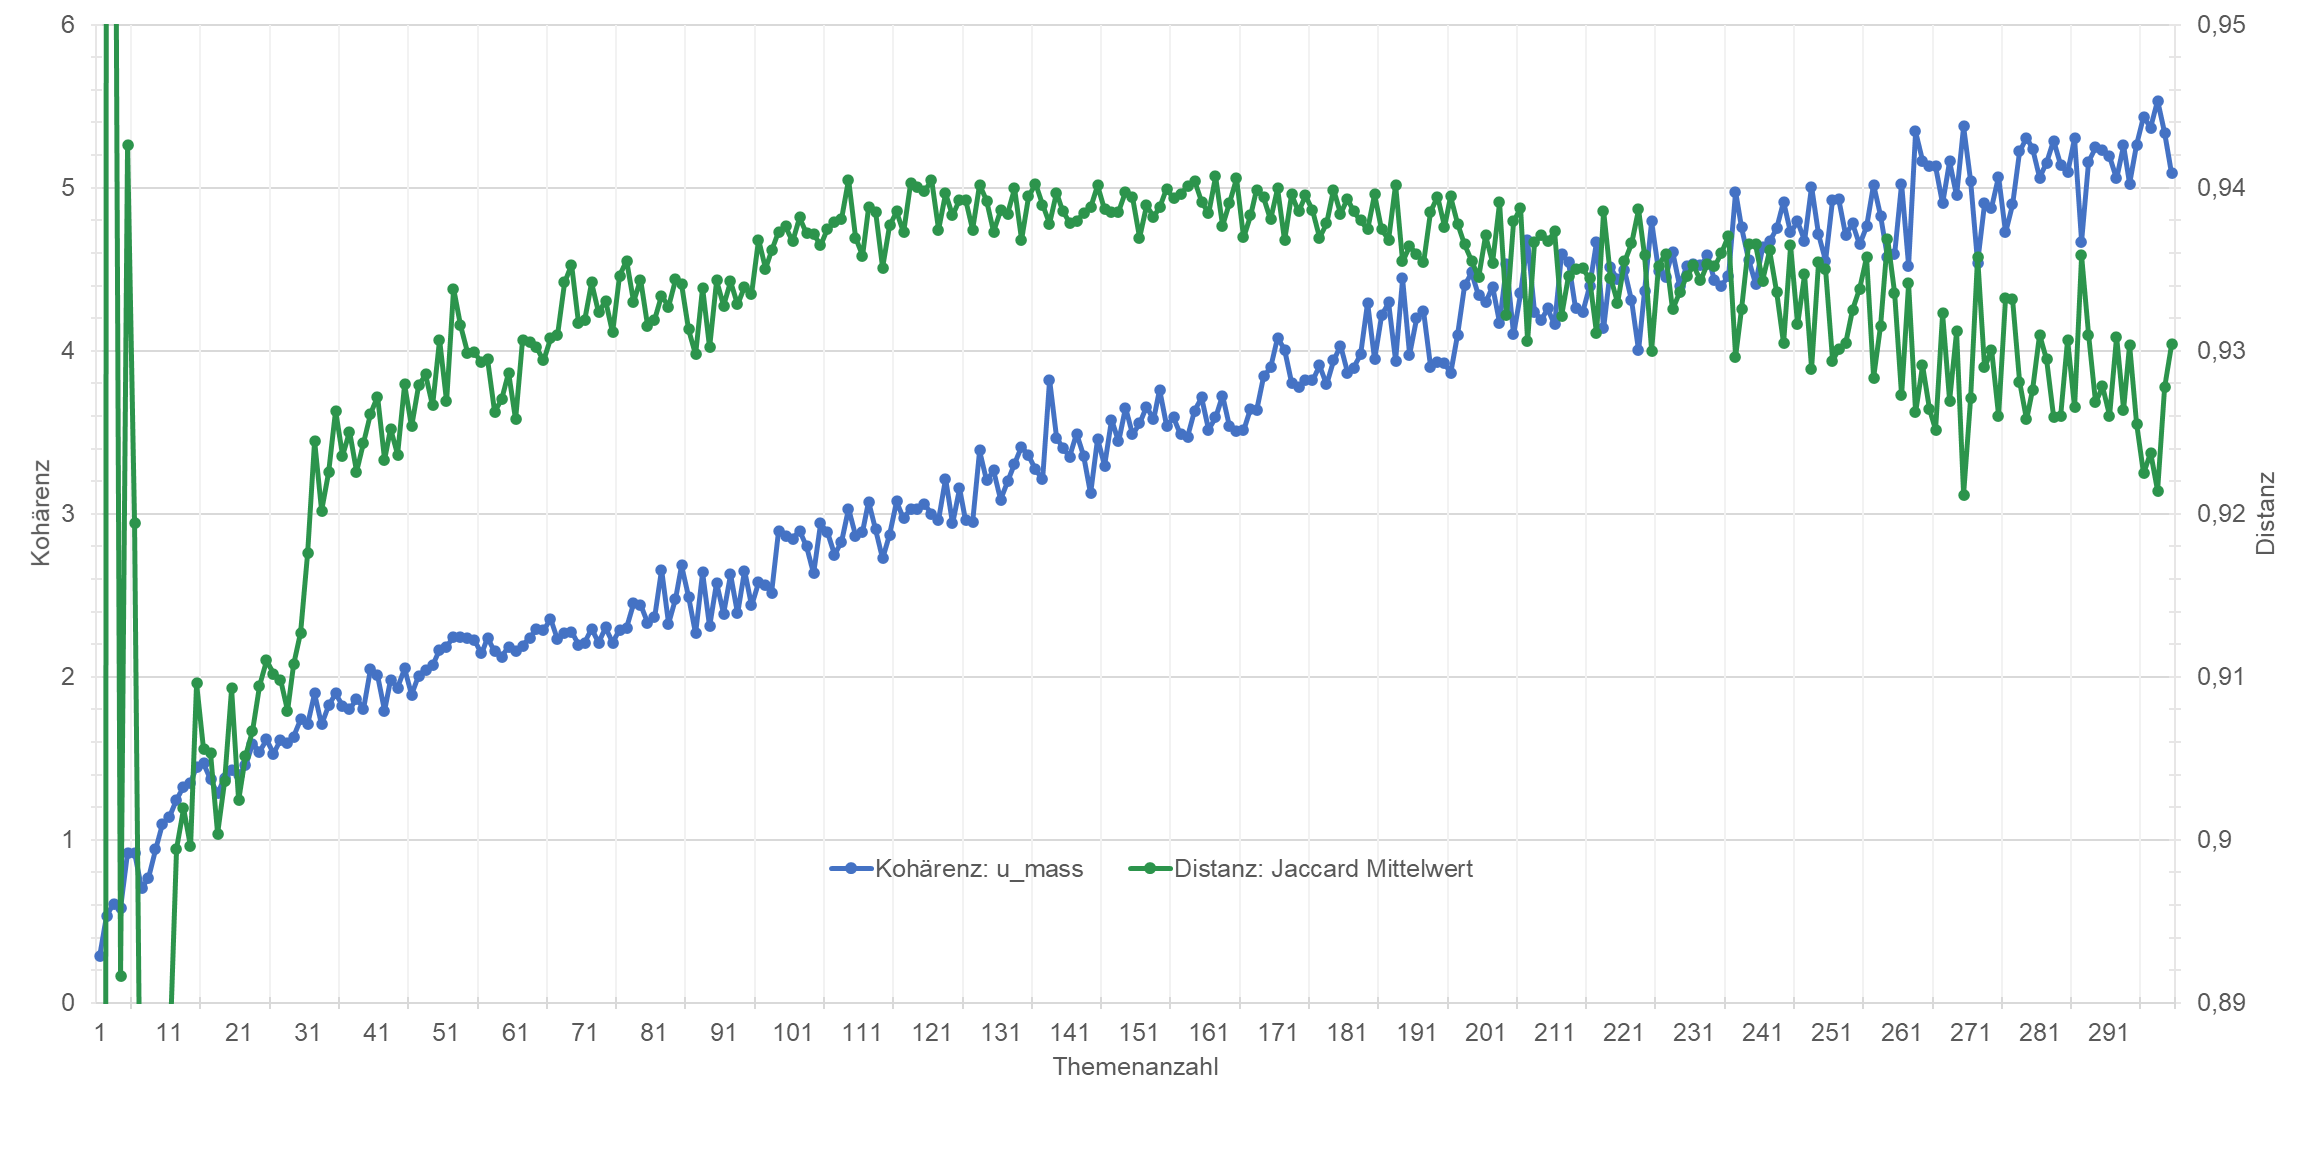
\includegraphics[width=\textwidth,height=10cm,keepaspectratio=true]{img/coherenceAndDistanceUnigram.png}
	\caption{
		Kohärenz und Distanz der Themen mit Unigrammen
	}
	\label{fig:Kohärenz_Distanz_Unigramme}
\end{figure}

Die Kohärenz der LDA Modelle wird mit dem u\_mass Maß bestimmt. Von eins wird der absolute u\_mass Wert vom LDA Modell mit n Themen subtrahiert und durch den absoluten u\_mass Wert des LDA Modells mit n + 1 Themen dividiert. Diese Berechnung wird für jedes Modell durchgeführt. Dadurch lässt sich die größte absolute Kohärenzsteigerung zum Vorgänger finden.

\begin{center}
	$1-\frac{\left|LDA n\right|}{\left|LDA n + 1\right|}$ 
\end{center}


Bei den Unigrammen sind es in Abbildung \ref{fig:Kohärenz_Distanz_Unigramme} 83 Themen. Bei den Bigrammen funktioniert diese Methode nicht so gut, um ein Plateau zu finden. Sie schlägt zehn Themen vor, was zu einem sehr groben Modell führt. Wie die Abbildung \ref{fig:Kohärenz_Distanz_Bigramme} zeigt wird eine hohe Kohärenz und Distanz bei der Themenanzahl von 51 erreicht. Mit der Anzahl wurde ein deutlich granulareres Modell erstellt. 

\begin{figure}[htpb]
	\centering
	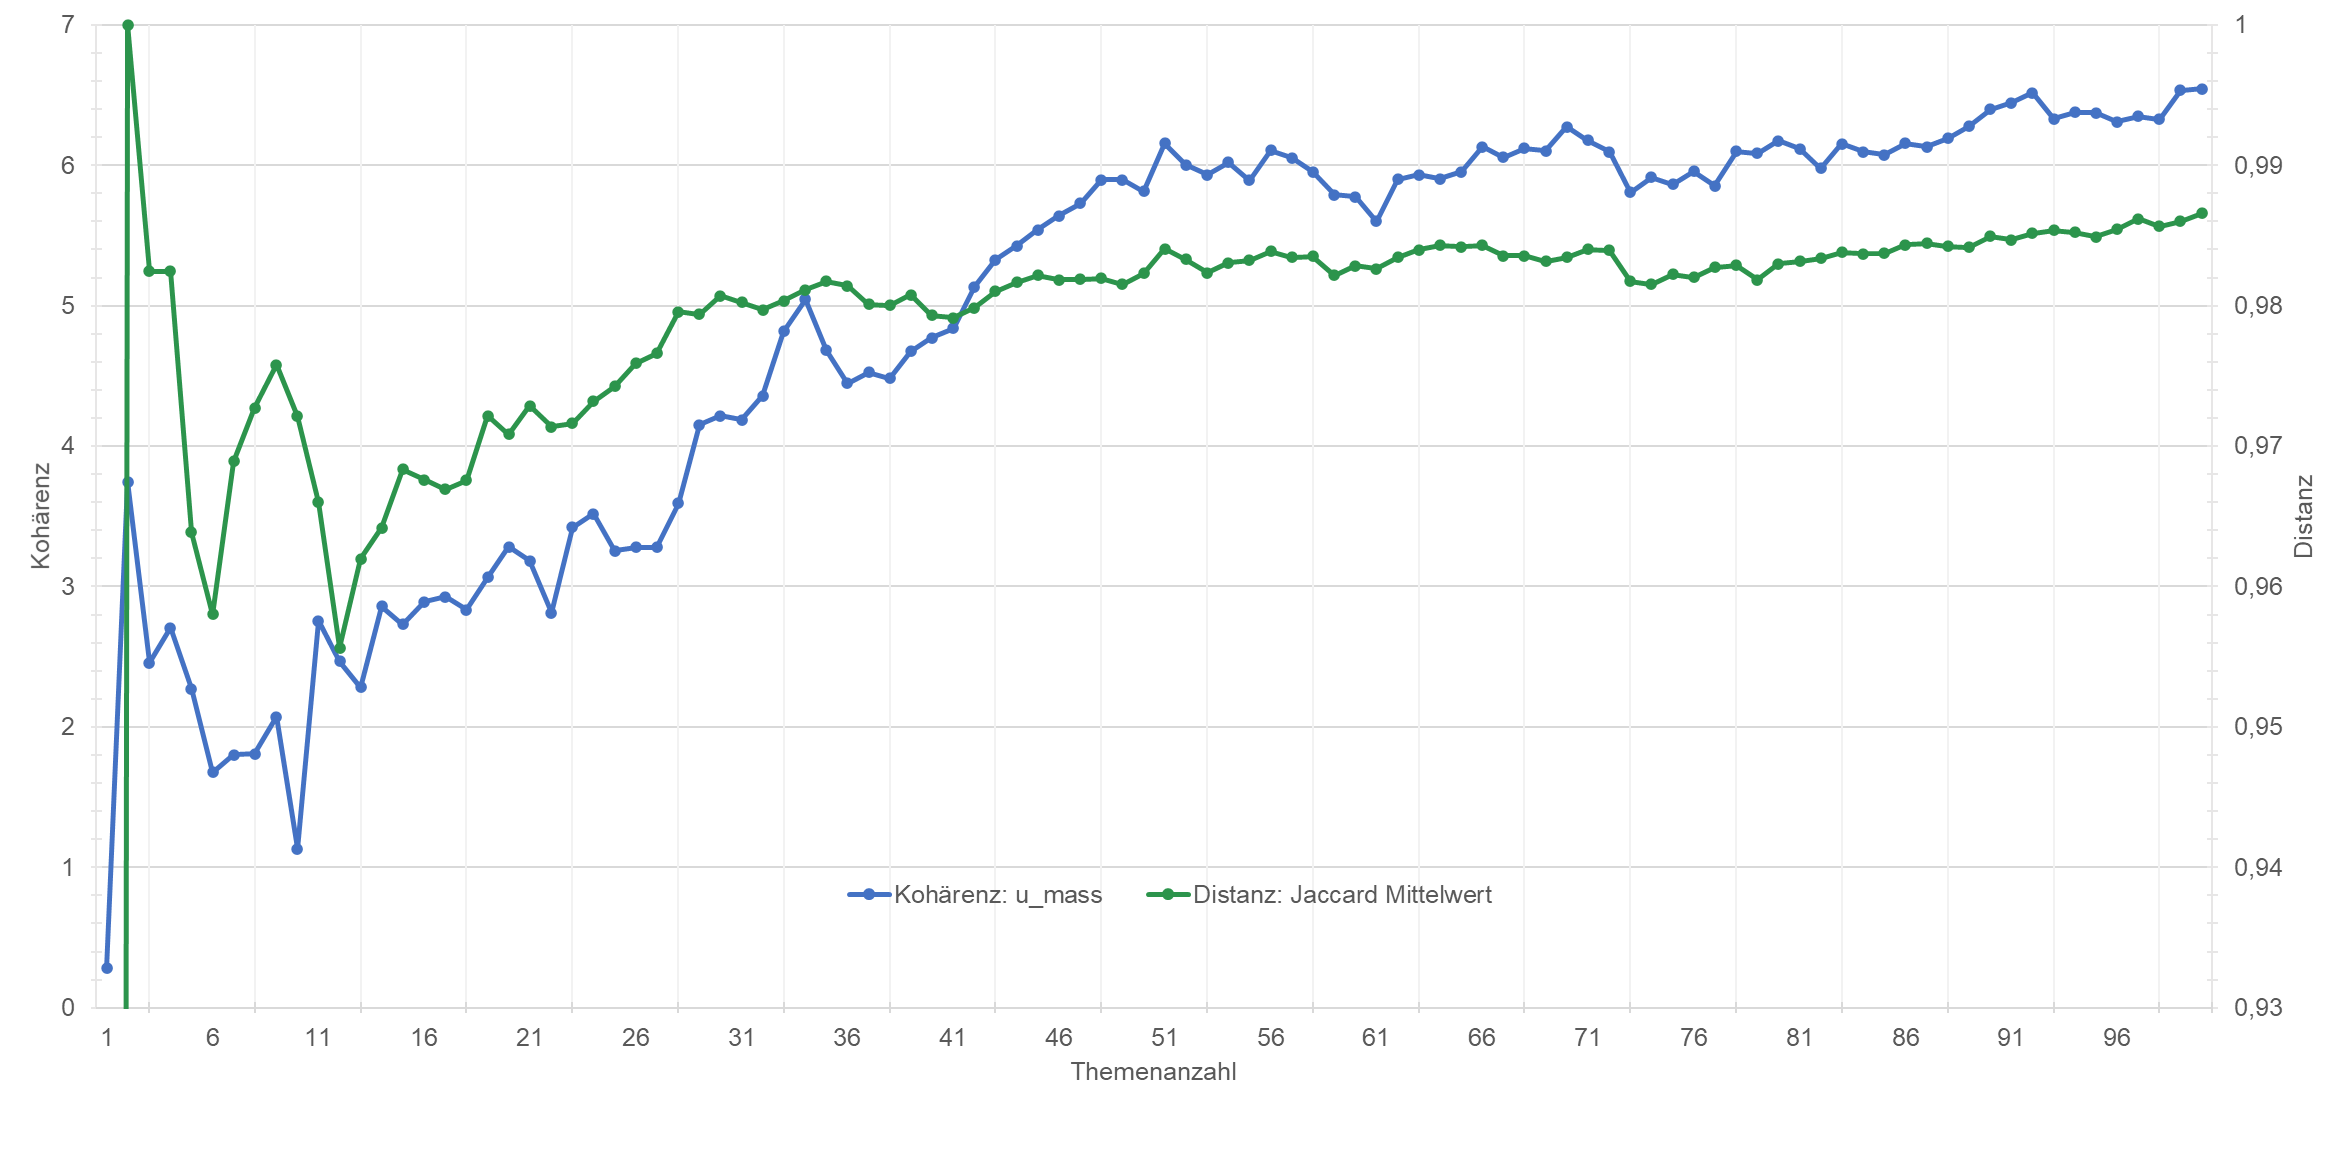
\includegraphics[width=\textwidth,height=10cm,keepaspectratio=true]{img/coherenceAndDistanceBigram.png}
	\caption{
		Kohärenz und Distanz der Themen mit Bigrammen
	}
	\label{fig:Kohärenz_Distanz_Bigramme}
\end{figure}


 

Im letzten Schritt werden die Daten als Themenliste, Dokument-Themen und Themen-Wort Matrizen gespeichert. Mit  pyLDAvis wird eine interaktive multidimensional skalierte Visualisierung erstellt. Diese Visualisierung berücksichtigt die Distanz und die Größe der Themen.


\subsection{Tomotopy}
Tomotopy ist ebenfalls eine Python library für Textanalyse. Sie ist ähnlich zu Gensim aber ist besonders performant und unterstützt zusätzlich \ac{hlda}, allerdings keine Kohärenzmaße. Deshalb werden hier beide librarys verwendet, um die jeweiligen Funktionen zu nutzen.

Die Wörter der Dokumente werden in eine Liste aus Listen geladen. Für \ac{hlda} wird keine Themenanzahl benötigt aber einige Parameter aus der Tabelle \ref{table:HLDA_Parameter} die \ac{lda} in Gensim selbst erlernt. Der \ac{hlda} verwirft die ersten 10.000 Iterationen und erstellt danach zehn Modelle mit einem Abstand von jeweils 100 Iterationen. \parencite[vgl.][S. 6]{griffiths2004hierarchical} \todo[inline]{25 random restarts to avoid local maxima, take highest posterior likelihood} In Abbildung \ref{fig:HLDA_Unigram_Baum} hat sich ein drei Ebenen tiefes Baumdiagramm als übersichtlich erwiesen, um Überthemen zu finden und Unterthemen zu clustern.

\begin{table}
	\centering
	\caption{HLDA Parameter}
	\begin{tabular}{|c|c|c|c|c|c|c|c|c|c|}
		\hline 
		Name& iterations & seed & TermWeight & $\alpha$ & $\eta$ & $\gamma$ & depth & rm\_top & burn\_in \\ 
		\hline 
		Unigrame& 1000 & 100 & \ac{tf-idf} & 0,3 & 0,6 & 0,15 & 3 & 1 & 10.000 \\ 
		\hline 
		Bigramme& 1000 & 100 & \ac{tf-idf} & 0,3 & 0,6 & 0,15 & 3 & 1 & 10.000  \\ 
		\hline  
	\end{tabular}
	\label{table:HLDA_Parameter}
\end{table} 

Die Term Frequency-Inverse Document Frequency (\ac{tf-idf}) wird benutzt, um herauszufinden wie relevant ein Wort für ein Dokument ist in einer Menge von Dokumenten. Der wert steigt proportional zu der Frequenz des Wortes in einem Dokument und sinkt mit der Anzahl an Dokumenten in denen das Wort vorkommt.

\begin{figure}[htpb]
	\centering
	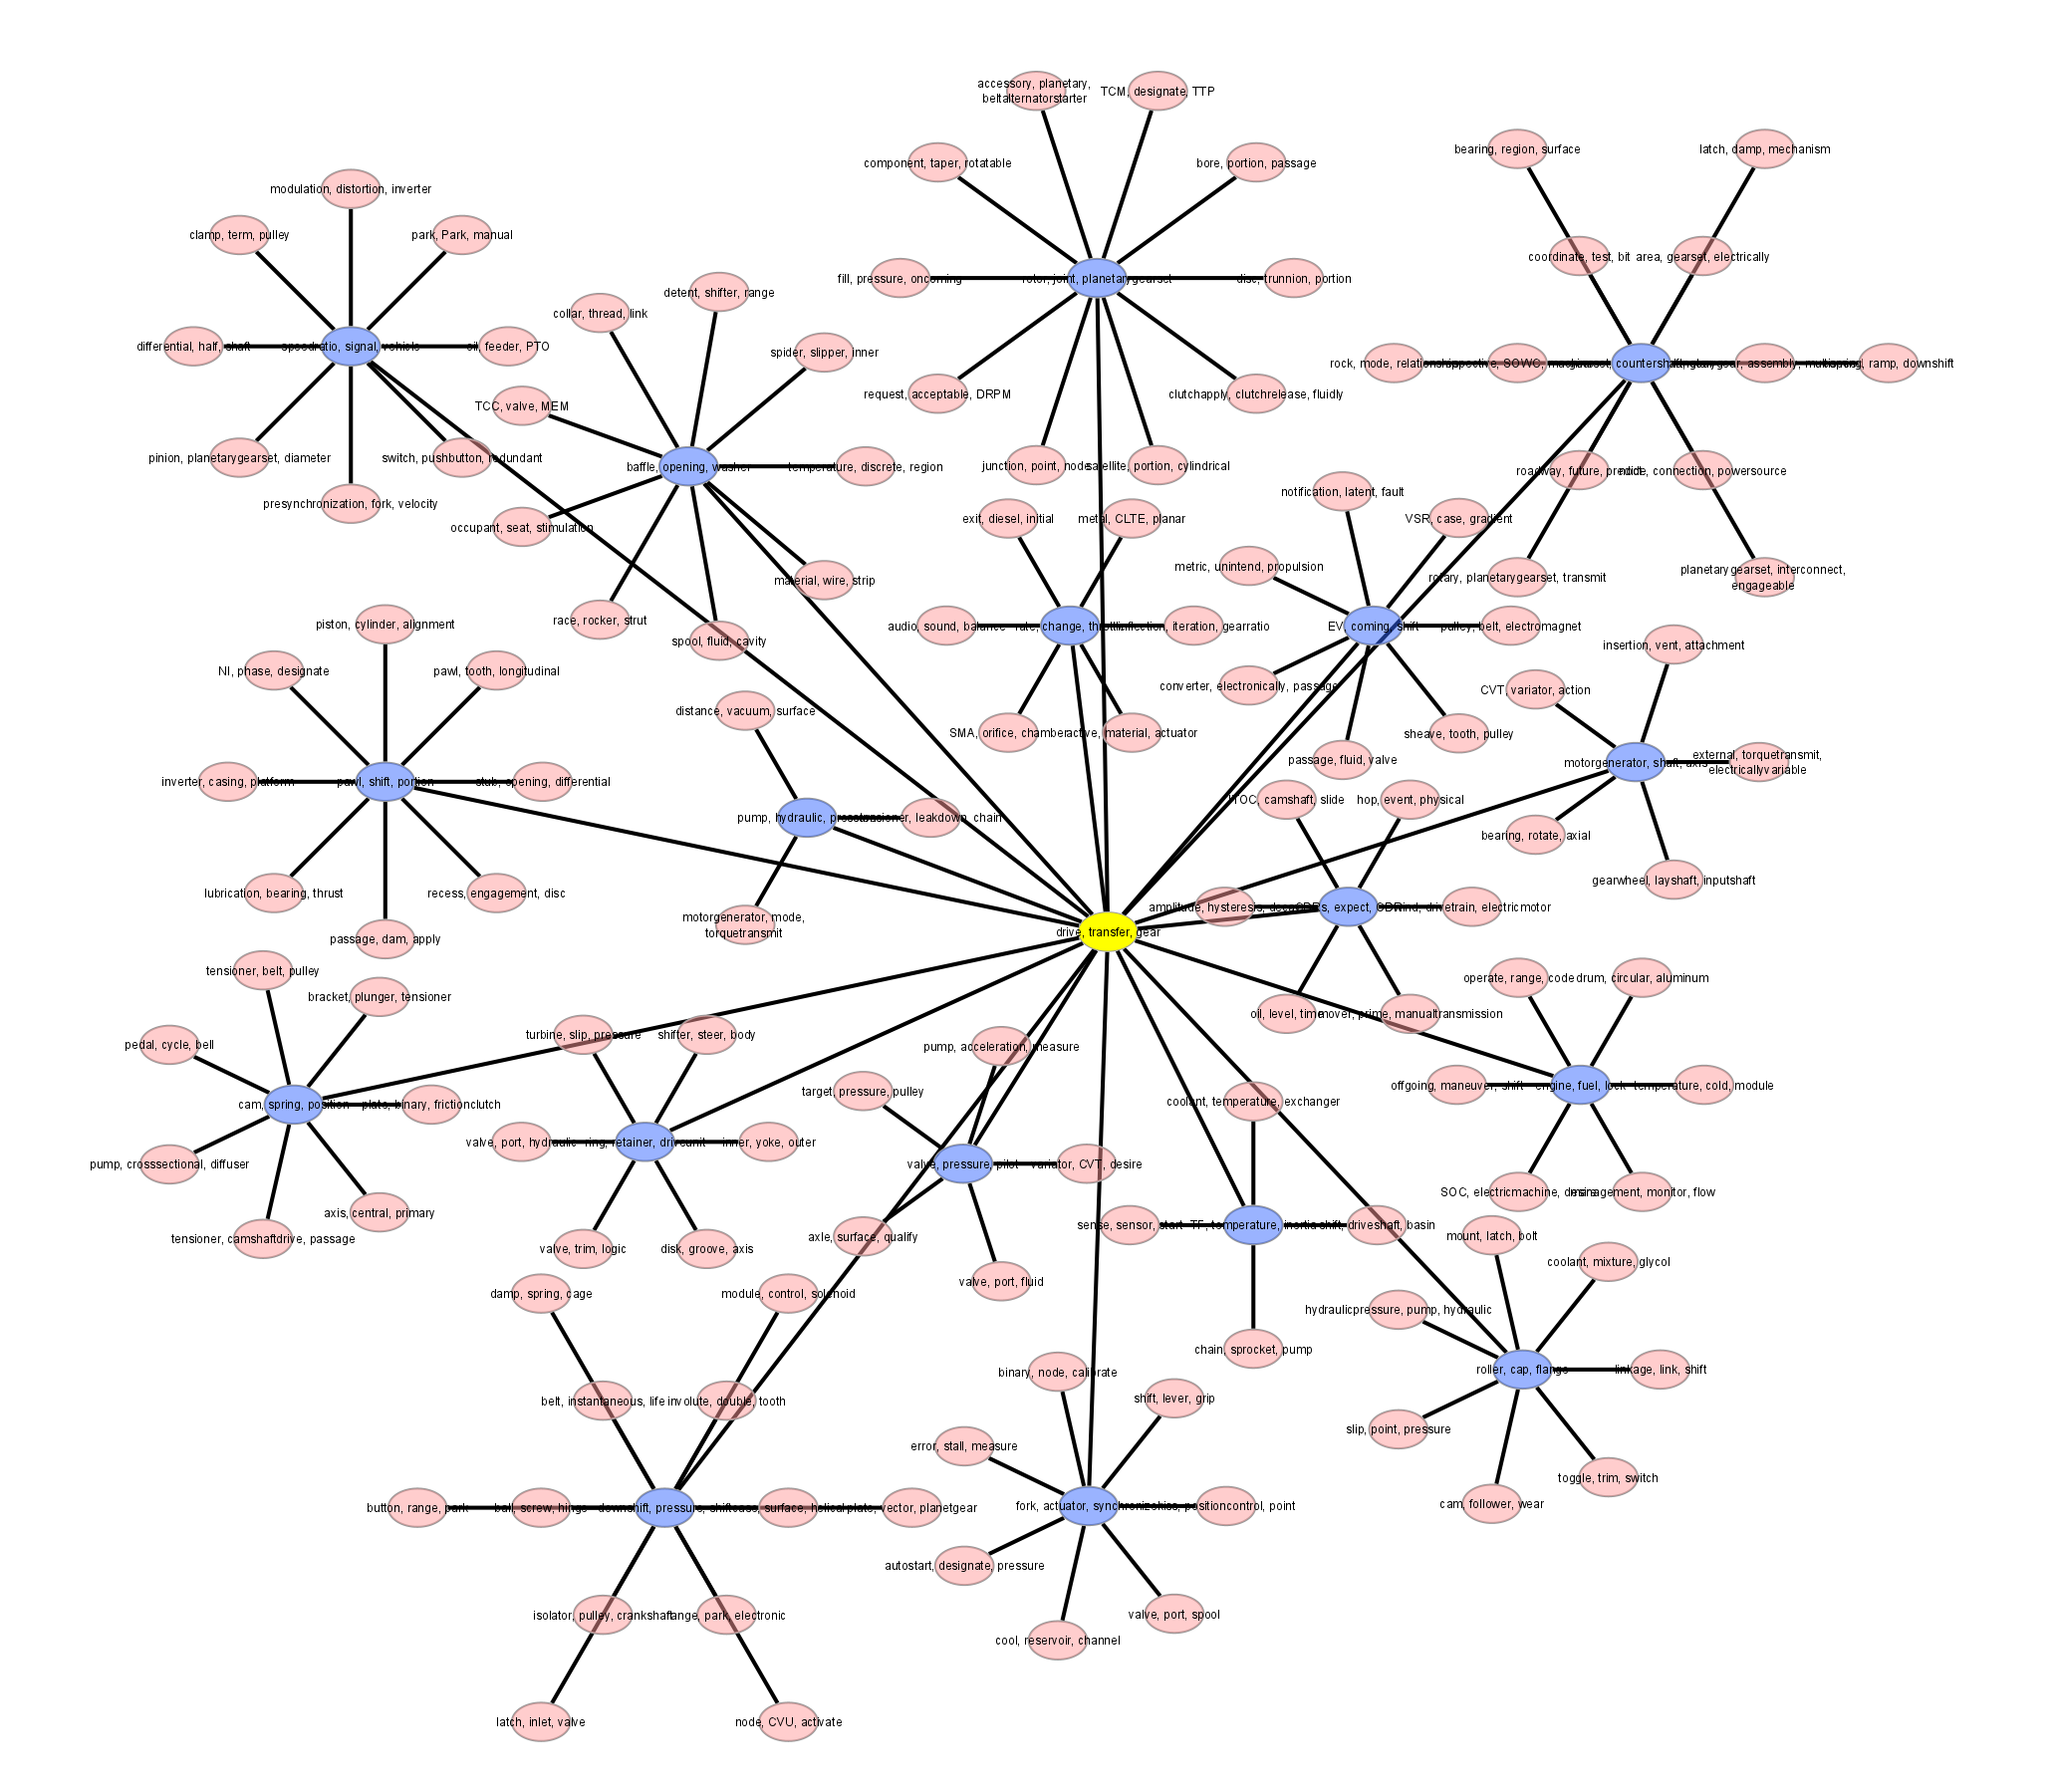
\includegraphics[height=15cm,width=\textwidth,keepaspectratio=true]{img/tree.png}
	\caption{
		HLDA Unigram Baumdiagramm
	}
	\label{fig:HLDA_Unigram_Baum}
\end{figure}

%\section{Gibbs Sampling}



\chapter{Analyse der Ergebnisse}


Die Analyse der Ergebnisse erfolgt in vier Schritten. Die Ergebnisse der drei Algorithmen werden einzeln ausgewertet und anhand markanter Beispiele erläutert. Mit dem \gls{lda} werden die latenten Themen und Themencluster des Patentdatensatzes benannt und eingegrenzt. Mit dem \gls{hlda} werden die gefundenen Themencluster bestätigt. Der \gls{dlda} wird die Entwicklung der relevantesten Themen über die Zeit beschreiben. Abschließend werden die Ergebnisse anhand von Kennzahlen verglichen.


%Kohärenz, Distanz, Themenanzahl, Verständlichkeit, Aufwand
\section{Analyse der Ergebnisse des \gls{lda}} \label{lda_analysis}

Zuerst werden die vier Schritte des qualitativen Verfahrens zur Benennung und Gruppierung der Themen aufgelistet. Danach werden die Schritte an Beispielen erklärt und wie das Verfahren durch quantitative Daten vom \gls{lda} unterstützt wird. Dies wird mit Abbildungen aus \gls{pyLDAvis} verdeutlicht. Die interaktive Version von \gls{pyLDAvis} befindet sich im digitalen Anhang. Danach werden die Themen benannt und gruppiert.

Das Verfahren zur Benennung und Gruppierung der Themen besteht aus vier Schritten:
\begin{enumerate}
	\item In \gls{pyLDAvis} Themencluster auswählen
	\item Die relevantesten Terme der Themen nacheinander auswählen
	\item Themenradien beobachten und Terme die in fast allen Themen des ausgewählten Clusters häufig vorkommen aber außerhalb nur selten vorkommen benennen den Cluster
	\item Bei diesem Vorgehen werden häufig Subcluster entdeckt, die ebenfalls nach dieser Methode benannt werden
\end{enumerate}

Die Themen welche durch \gls{lda} gefunden wurden, werden mit Hilfe von \gls{pyLDAvis} benannt und visualisiert \parencite[vgl.][S. 63]{sievert2014ldavis}. \gls{pyLDAvis} ist ein Programm, das die Themen multidimensional skaliert und interaktiv darstellt. In Abbildung \ref{fig:clustering_process01} werden links die Themenradien nach Termanzahl skaliert. Die Tabelle rechts zeigt die Termhäufigkeiten im ausgewählten Thema Nummer 50 und im gesamten Korpus.

\begin{landscape}
 \begin{figure}[htpb]
	\centering
	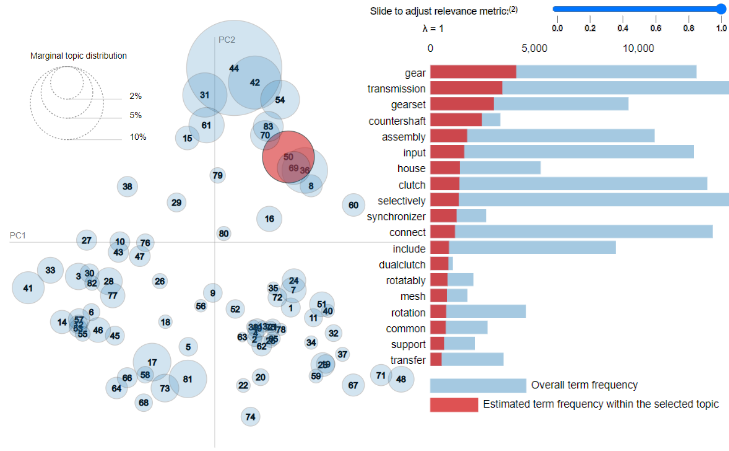
\includegraphics[width=19.29cm,keepaspectratio=true]{img/clustering_process01.png}
	\caption{
		Interthematische Distanz Karte erstellt mit multidimensionaler Skalierung und die relevantesten Terme für das Thema Nummer 50 bei einem $\lambda = 1,0$
	}
	\label{fig:clustering_process01}
 \end{figure}
\end{landscape}

 
 
In Abbildung \ref{fig:clustering_process02} wurde das $\lambda$ von $1,0$ auf $0,6$ herabgesetzt. Dadurch werden die Terme im ausgewählten Thema absteigend nach Relevanz sortiert. Der Parameter $\lambda$ soll mit dem Wert $0,6$ den Anwender die korrektesten  Themen finden lassen \parencite[vgl.][S. 66-68]{sievert2014ldavis}. Rechts wurde der Term \emph{countershaft} ausgewählt. Dadurch werden die Themenradien, abhängig von der Verteilung des ausgewählten Terms, skaliert. Die Themen 50, 20 und 83 enthalten die meisten der \emph{countershaft} Terme und sind teil des pink eingekreisten Subcluster des \emph{transmission} Clusters, aus Abbildung \ref{fig:Themengruppen_LDA_Unigramm}. Deshalb sind sie als \emph{countershaft} Themen zu werten.

\begin{landscape}
	\begin{figure}[htpb]
		\centering
		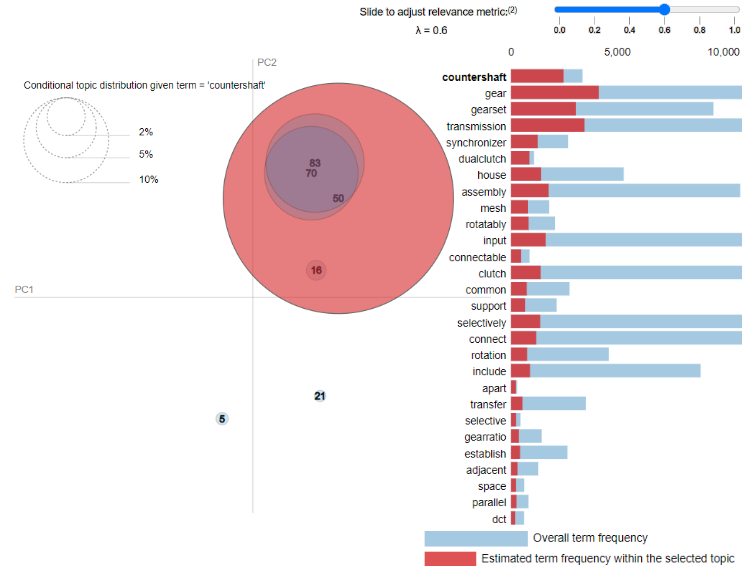
\includegraphics[width=19.29cm,keepaspectratio=true]{img/clustering_process02.png}
		\caption{
			Interthematische Distanz Karte erstellt mit multidimensionaler Skalierung mit einer Themenverteilung welche von dem Term countershaft abhängt und die relevantesten Terme für das Thema Nummer 50 bei einem $\lambda = 0,6$ 
		}
		\label{fig:clustering_process02}
	\end{figure}
\end{landscape}

 
Außerdem kommen die äquivalenten Terme \emph{dualclutch}, \emph{dct} und \emph{automatictransmission} besonders häufig in den Themen 50, 83, 69 und 10 vor. Das ist ein weiterer Teil des Subclusters \emph{transmission}. Des weiteren sind die Terme \emph{synchronizer} und \emph{mesh} beide in den Themen 50, 70 und benachbarten Themen häufig zu finden. Das deutet auf das synchronisieren der \emph{shafts} hin. Durch dieses qualitative Verfahren werden die Themen benannt und Cluster gebildet. Doch \gls{pyLDAvis} reicht allein nicht immer aus. Thema 77 deutet mit den Termen \emph{clutch} und \emph{slip} auf eine Slipper clutch hin aber warum befindet es sich dann in dem \emph{method} Cluster? Für genauere Einblicke in Themen wurde mit \gls{lda} eine Patent-Themen-Matrix erstellt. Das Patent 9,989,146 passt am besten zu Thema 77. Es beschreibt eine Methode, welche den optimalen Druck einer \emph{clutch} in einem \gls{cvt} erlernt, damit die sie einen \emph{pulley slip} verhindern kann. Daher kommt in diesem Thema der Term \emph{pressure} ohne \emph{fluid} oder \emph{hydraulik} vor.
 
 \begin{figure}[htpb]
 	\centering
 	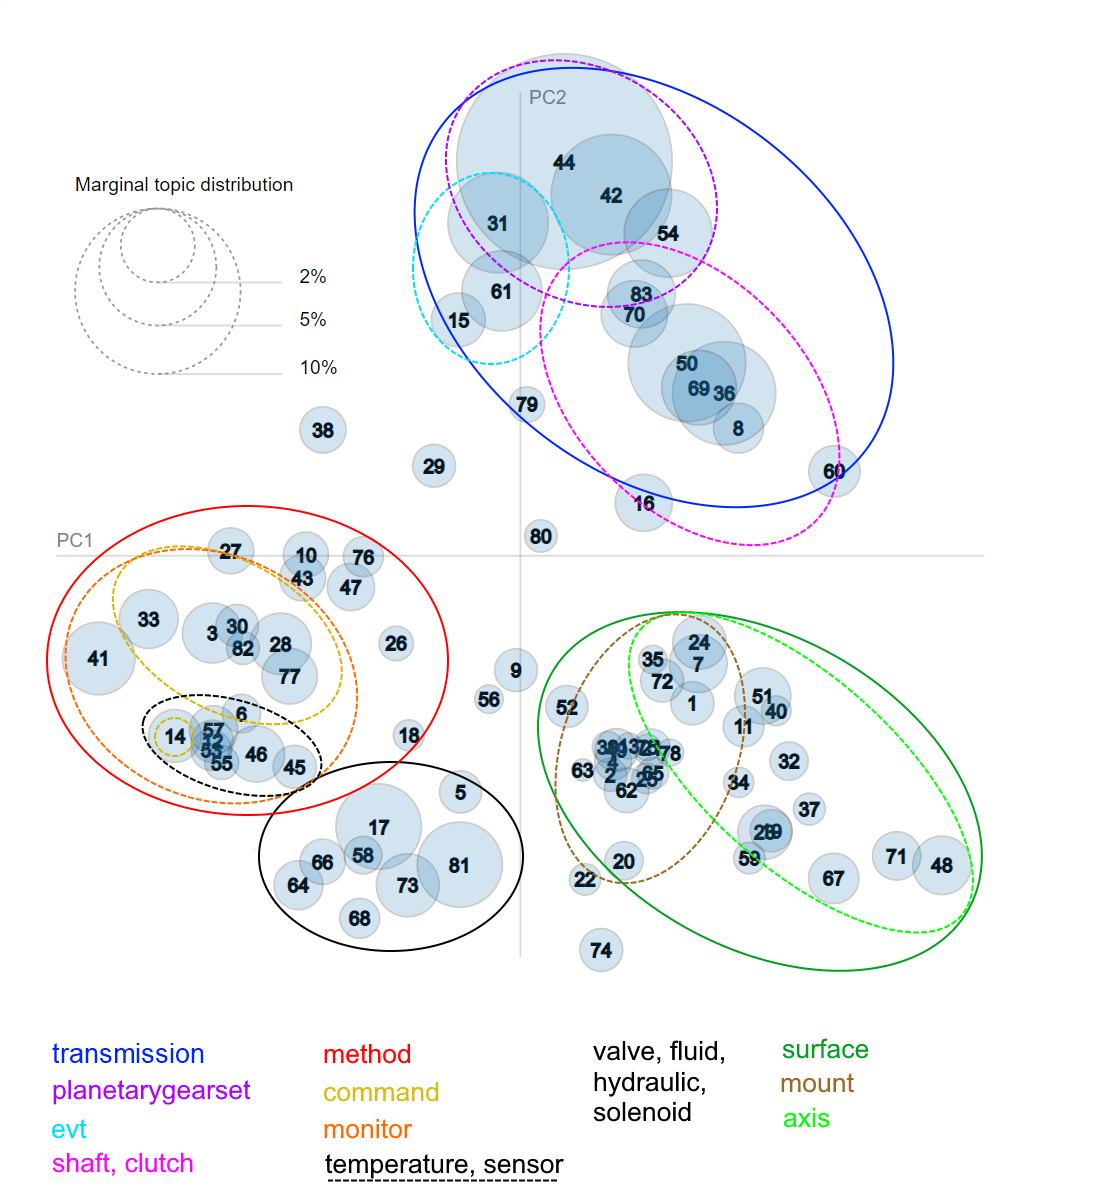
\includegraphics[width=\textwidth,keepaspectratio=true]{img/LDAvisGM-3-1-1_clustered.png}
 	\caption{
 		Themengruppen der LDA Unigramme multidimensionale Skalierung
 	}
 	\label{fig:Themengruppen_LDA_Unigramm}
 \end{figure}
 
 
Der blaue Cluster besteht hauptsächlich aus Themen zu \emph{transmission} Komponenten. Fast alle Themen des blauen Clusters enthalten die Terme \emph{transmission}, \emph{sungear} und \emph{ringgear}. Der lila Subcluster enthält das größte Thema des Datensatzes Nummer 44. Die Themen beinhalten das \emph{planetarygearset}, die \emph{multispeedtransmission} und werden zum \emph{torquetransmit} genutzt. Der türkise Cluster zeigt das Thema \gls{evt} mit einem \emph{motorgenerator} für Hybridautos. Der pinke Cluster beinhaltet die \emph{dualclutch}, die  \emph{automatictransmission}, den \emph{countershaft}, den \emph{inputshaft} und die \emph{synchronizer} welche die \emph{shafts} verbinden (\emph{mesh}). Dies wird im Patent 8,240,224 beschrieben.
 
Der Rote Cluster enthält besonders viele Terme wie \emph{method}, \emph{command} und \emph{request}. Der Cluster besteht daher aus Steuerungs- und Regelungsthemen von Fahrzeugen.
 
Im gelben Subcluster geht es hauptsächlich um die elektronische Steuerung von Kupplungen, dem Motor und dem \gls{cvt}. Er ist eine Teilmenge des orangen Subclusters, weil in dem gelben Subcluster viel häufiger der Term \emph{command} vorkommt und \emph{montior} gleichmäßiger im gesamten orangen Subcluster einschließlich des gelben Subclusters verteilt ist. Das Thema Nummer 14 ist eine Ausnahme, weil es fast gleich viele Terme von \emph{command} und \emph{monitor} für die \emph{hydraulic} \emph{pressure} enthält. Deshalb ist es extra gelb umkreist. Die \emph{frictionclutch} ist hauptsächlich dem Thema 77 zuzuordnen. Der Term \emph{slip} kommt in Verbindung mit der \emph{clutch} in den umliegenden Themen häufig vor. Auch die \emph{dogclutch} ist in dem gelben Subcluster zu finden obwohl sie hauptsächlich im Thema 5 vorkommt. Im Thema 28 geht es um die Steuerung der \emph{binary} \emph{clutch} (9,061,675), die im Thema 50 schon \emph{dualclutch} genannt wurde. Das Thema 3 umfasst das besagte \gls{cvt}. Fast alle Themen des roten Clusters sind eng verbunden mit dem \emph{engine}, besonders die Themen 41 und 33.
 
Der schwarze Subcluster enthält viele Themen zur Beobachtung (\emph{monitor}, \emph{sensor}) der \emph{temperature} und der \emph{pressure}. In diesem schwarzen Subcluster geht es hauptsächlich um Themen die mit Flüssigkeit in Verbindung stehen. Es geht um die \emph{hydraulic} \emph{pressure} (14), die \emph{hydraulic} \emph{pump} (45) und die \emph{temperature} des \emph{coolant} im Kühlkreislauf der \emph{electricmachine} (8,167,773), der \emph{engine} und des \emph{radiator} (57). Durch die Steuerung des Kühlkreislauf können Komponenten wie die \emph{transmission} auf Betriebstemperatur gebracht werden (10,161,501). Zu dem Thema 12 passt am besten das Patent 9,404,403, es beschreibt eine Methode um das Öllevel zu beobachten (\emph{monitor}). Auf Grund der vielen Flüssigkeitsthemen befindet sich der schwarze Subcluster in der Nähe des schwarzen Hauptclusters.
 
Der schwarze Hauptcluster enthält fast alle Themen die in Verbindung mit Flüssigkeit stehen. Er teilt die Häufigkeit des von \emph{control} mit dem roten Cluster aber unterscheidet sich durch die Verwendung von die Terme \emph{communication} und \emph{communicate} die sonst nur selten auftreten. Besonders häufig ist die Kombination \emph{solenoid}, \emph{hydraulic}, \emph{valve} und \emph{fluid}. Das Thema 17 beschreibt in mehreren Patenten (8,820,185
, 8,382,639) die Steuerung einer \emph{dualclutch} mithilfe von \emph{hydraulic} und \emph{solenoids}. Mit einem Elekrtomagnet (\emph{solenoids}) wird ein Verschluss aus der \emph{valve} gezogen. Dieser Verschluss wird nach dem nach dem Ausschalten des \emph{solenoids} mit einer Feder zurück in die \emph{valve} geschoben. Mit einem \emph{solenoid} kann auch Druck erzeugt werden. Daher kommt der Term \emph{pressure} ebenfalls häufig vor. Diese Methode findet Verwendung in Thema 68, dort wird beschrieben wie eine \emph{actuator} \emph{fork} kontrolliert (\emph{control}) werden kann (9,605,755).

Der dunkel grüne Cluster besteht aus sehr vielen kleinen Themen die nicht gänzlich durch thematische Nähe gruppiert wurden. Ein gemeinsamer Term ist \emph{bias} was auf Zahnräder hindeutet. Das ist leider unspezifisch. Der hellgrüne Subcluster hingegen hat zwei beschreibende Terme. \emph{shaft}, \emph{axis} und \emph{house} zeigen eine Verwandschaft mit dem pinken Subcluster, der ebenfalls \emph{shaft} \emph{house} enthält. Das \emph{house} deutet auf das gear housing hin was auch zu den Termen \emph{surface}, \emph{side} und \emph{body} passt die den gesamten dunkelgrünen Cluster bilden.
 
 
%\todo[inline]{DVU, TCM, ECM, VSR, DCT, ETR? gelber cluster}
 
%Der orange Subcluster 
 
 
 
%9 layshaft
%52 turbine
 
 


\section{Analyse der Ergebnisse des \gls{hlda}}

Die Ergebnisse des \gls{hlda} werden im Vergleich mit den \gls{lda} Ergebnissen analysiert. Zwei Subcluster des \gls{hlda} Baums werden mit den Ergebnissen des \gls{lda} verglichen und analysiert. Der ganze \gls{hlda} Baum ist zu groß um leserlich abgebildet zu werden. Er kann im digitalen Anhang mit einem Programm geöffnet werden, das graphml unterstützt, zum Beispiel Cytoscape.

Der \emph{engine} Subcluster aus Abbildung \ref{fig:hlda_engine} passt gut zu dem orangefarbenen Subcluster aus der \gls{lda} Abbildung \ref{fig:Themengruppen_LDA_Unigramm}. Die Terme \emph{engine} und \emph{fuel} passen zu dem Motorthema 41. Die Subthema \emph{monitor} passt genau zu dem orangefarbenen Subcluster und \emph{temperature} gehört mit \emph{electricmachine} zum Thema 57. Dadurch werden die mit \gls{lda} benannten Themen bestätigt. Die Subthemen \emph{operate}, \emph{shift} und \emph{drum} sind im \gls{lda} Modell in dieser Form nicht in der Nähe aufzufinden. Allerdings passen sie thematisch zu den anderen.

\begin{figure}[htpb]
	\centering
	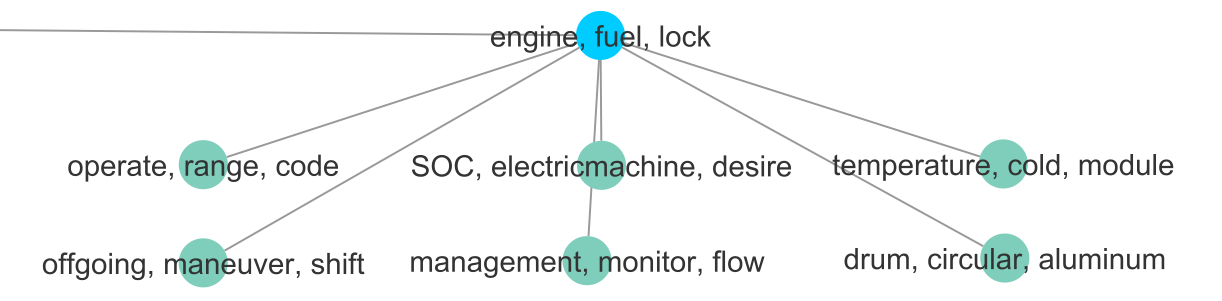
\includegraphics[width=\textwidth,keepaspectratio=true]{img/hldaEngine.png}
	\caption{
		Der \emph{engine} Ausschnitt des \gls{hlda} Baums
	}
	\label{fig:hlda_engine}
\end{figure}

Der \emph{fork} Subcluster aus Abbildung \ref{fig:hlda_fork} passt genau zu dem schwarzen Cluster aus Abbildung \ref{fig:Themengruppen_LDA_Unigramm}. Dort beschreibt das Thema 68 ebenfalls eine \emph{synchronizer actuator fork} aus dem Patent 9,605,755. Der \gls{hlda} Subcluster enthält außerdem die Subthemen \emph{valve}, \emph{spool}, \emph{cool}, \emph{pressure}, \emph{calibrate}, \emph{position} und \emph{control}. Diese kommen auch alle im \gls{lda} Cluster vor und bestätigen erneut die Ergebnisse. Die \emph{spool} ist eine Spule und daher ein Bestandteil des Elektromagneten \emph{solenoid}.

\begin{figure}[htpb]
	\centering
	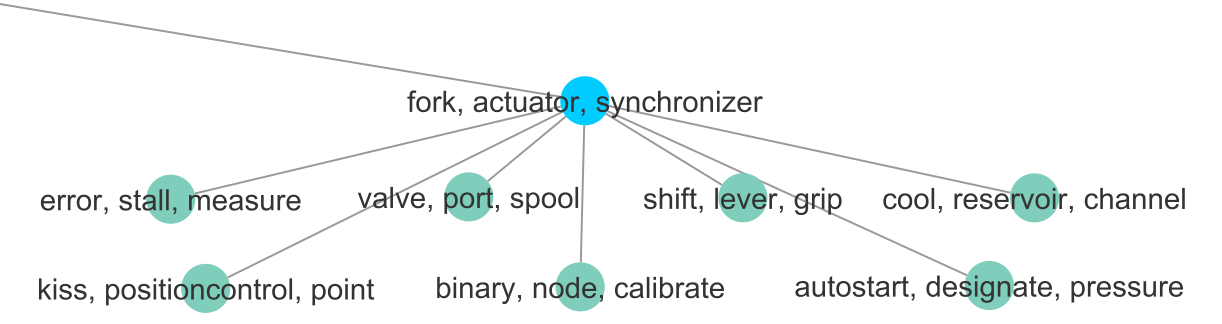
\includegraphics[width=\textwidth,keepaspectratio=true]{img/hldaFork.png}
	\caption{
		Der \emph{fork} Ausschnitt des \gls{hlda} Baums
	}
	\label{fig:hlda_fork}
\end{figure}


\section{Analyse der Ergebnisse des \gls{dlda}}

Die Ergebnisse des \gls{dlda} werden zuerst eingeordnet und die Wahl der Terme, welche die ausgewählten Cluster und Themen repräsentieren, erläutert. Dann werden die Trends der Terme festgestellt.

Der \gls{dlda} wurde mit den Ergebnissen des \gls{lda} und den Anmeldedaten der Patente gespeist. Daher sind die Ergebnisse des \gls{dlda} direkt vergleichbar mit denen des \gls{lda}. Die Terme wurden so gewählt, dass sie die Cluster möglichst genau beschreiben. Außerdem sollen sie relativ selten in anderen Clustern vorkommen, damit ihr Trend nicht verfälscht wird. Diese Bedingungen der Clusterbenennung wurden in \ref{lda_analysis} berücksichtigt.

Der größten Cluster heißt \emph{transmission}. In Abbildung \ref{fig:dlda_overall} verzeichnet er einen leichten Abwärtstrend. Der alternative Term \emph{selectively} bestätigt diesen Trend. Der pinke Subcluster  Deutlich stärker sinkt die relative Häufigkeit des Terms \emph{fluid}. Der Term \emph{valve} bestätigt die sinkende Zahl von Patentanmeldungen mit Bezug zu Flüssigkeiten. Die Häufigkeit verringerte sich von 2004 bis 2017 von 0,95\% auf 0,72\%. Der benachbarte Cluster \emph{method} gewinnt moderat an Häufigkeit. Er enthält hauptsächlich Patente mit Methoden zur elektronischen Steuerung und Regelung von mechanischen Bauteilen. Der Term \emph{command} bestätigt den Aufwärtstrend mit einer Erhöhung von 0,2\% auf 0,23\%. 



  \begin{figure}[!ht]
	\centering
	\begin{floatrow}
		\ffigbox[\FBwidth]{\caption{Trends der Terme die ihren Cluster am besten beschreiben}\label{fig:dlda_overall}}{%
			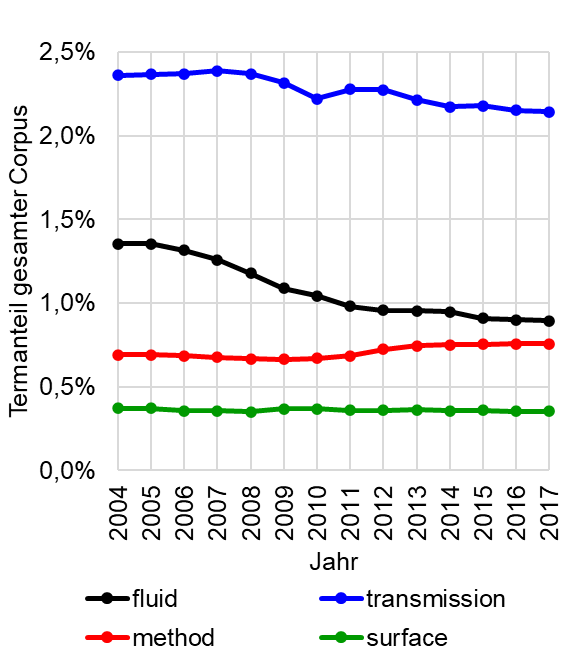
\includegraphics[width=\linewidth,keepaspectratio=true]{img/DLDA_overall.png}
		}
		\ffigbox[\FBwidth]{\caption{Trends der 3 Terme die das Thema 50 am besten beschreiben}\label{fig:dlda_topic_50}}{%
			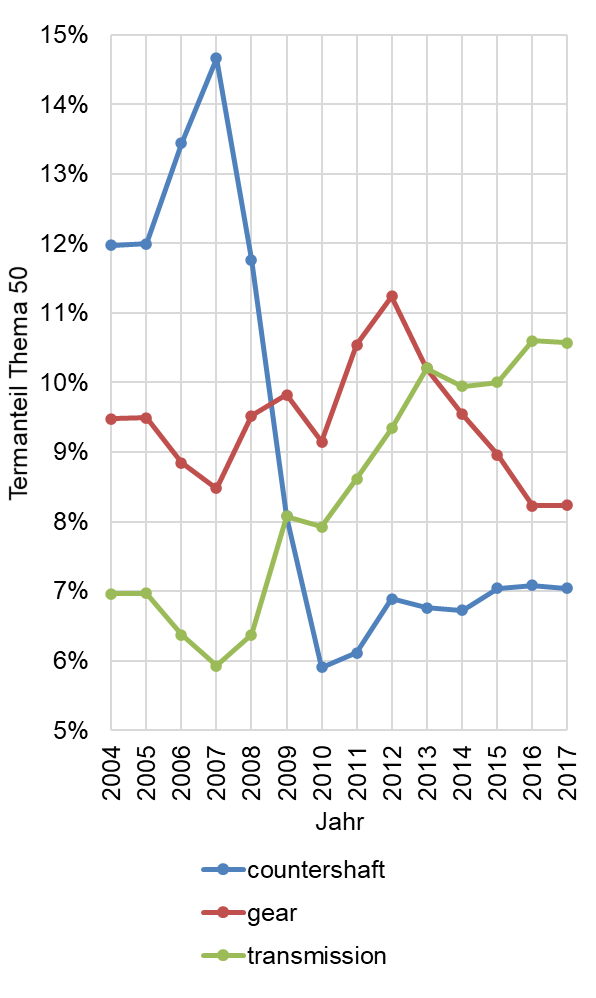
\includegraphics[width=\linewidth,keepaspectratio=true]{img/DLDA_topic_50.png}
		}
	\end{floatrow}
\end{figure}


\section{Vergleich der Ergebnisse anhand von Kennzahlen}
Die Unigrammmodelle weisen eine niedrigere Distanz zueinander auf als die Bigrammmodelle. Das liegt daran, das es deutlich mehr Bigramme gibt und diese auch als unterschiedlich gewertet werden wenn sie sich nur teilweise unterscheiden. Ein Beispiel wäre gear gearset und gear gear. In \ref{fig:Kohärenz_Distanz_Unigramme} wird ersichtlich das sich die Kohärenz mit steigender Themenzahl verbessert bis sie gleich der Anzahl an Wörtern im Datensatz ist. Die Distanz hingegen sinkt nachdem sie einen Hochpunkt erreicht. In Abbildung 4.1 sind Muster und Hotspots aus Unigrammthemen zu erkennen, die besonders ähnlich oder unähnlich sind. Diese werden später geclustered. In Abbildung 4.2 gibt es ebenfalls Muster und Hotspots. Allerdings sind manche Bigrammthemen disjunkt, wodurch sie eine Distanz von 1 haben. 

\begin{table}
	\RawFloats
	\centering
	\caption{Kohärenzen}
	\begin{tabular}{|c|c|c|}
		\hline
		Modell & Unigramm & Bigramm \\
		\hline
		LDA & -2,03 & -5,51 \\
		\hline
		HLDA & -4,30 & -5,90 \\
		\hline
	\end{tabular}
	\label{table:Kohärenzen}
\end{table} 

\begin{figure}[htpb]
	\centering
	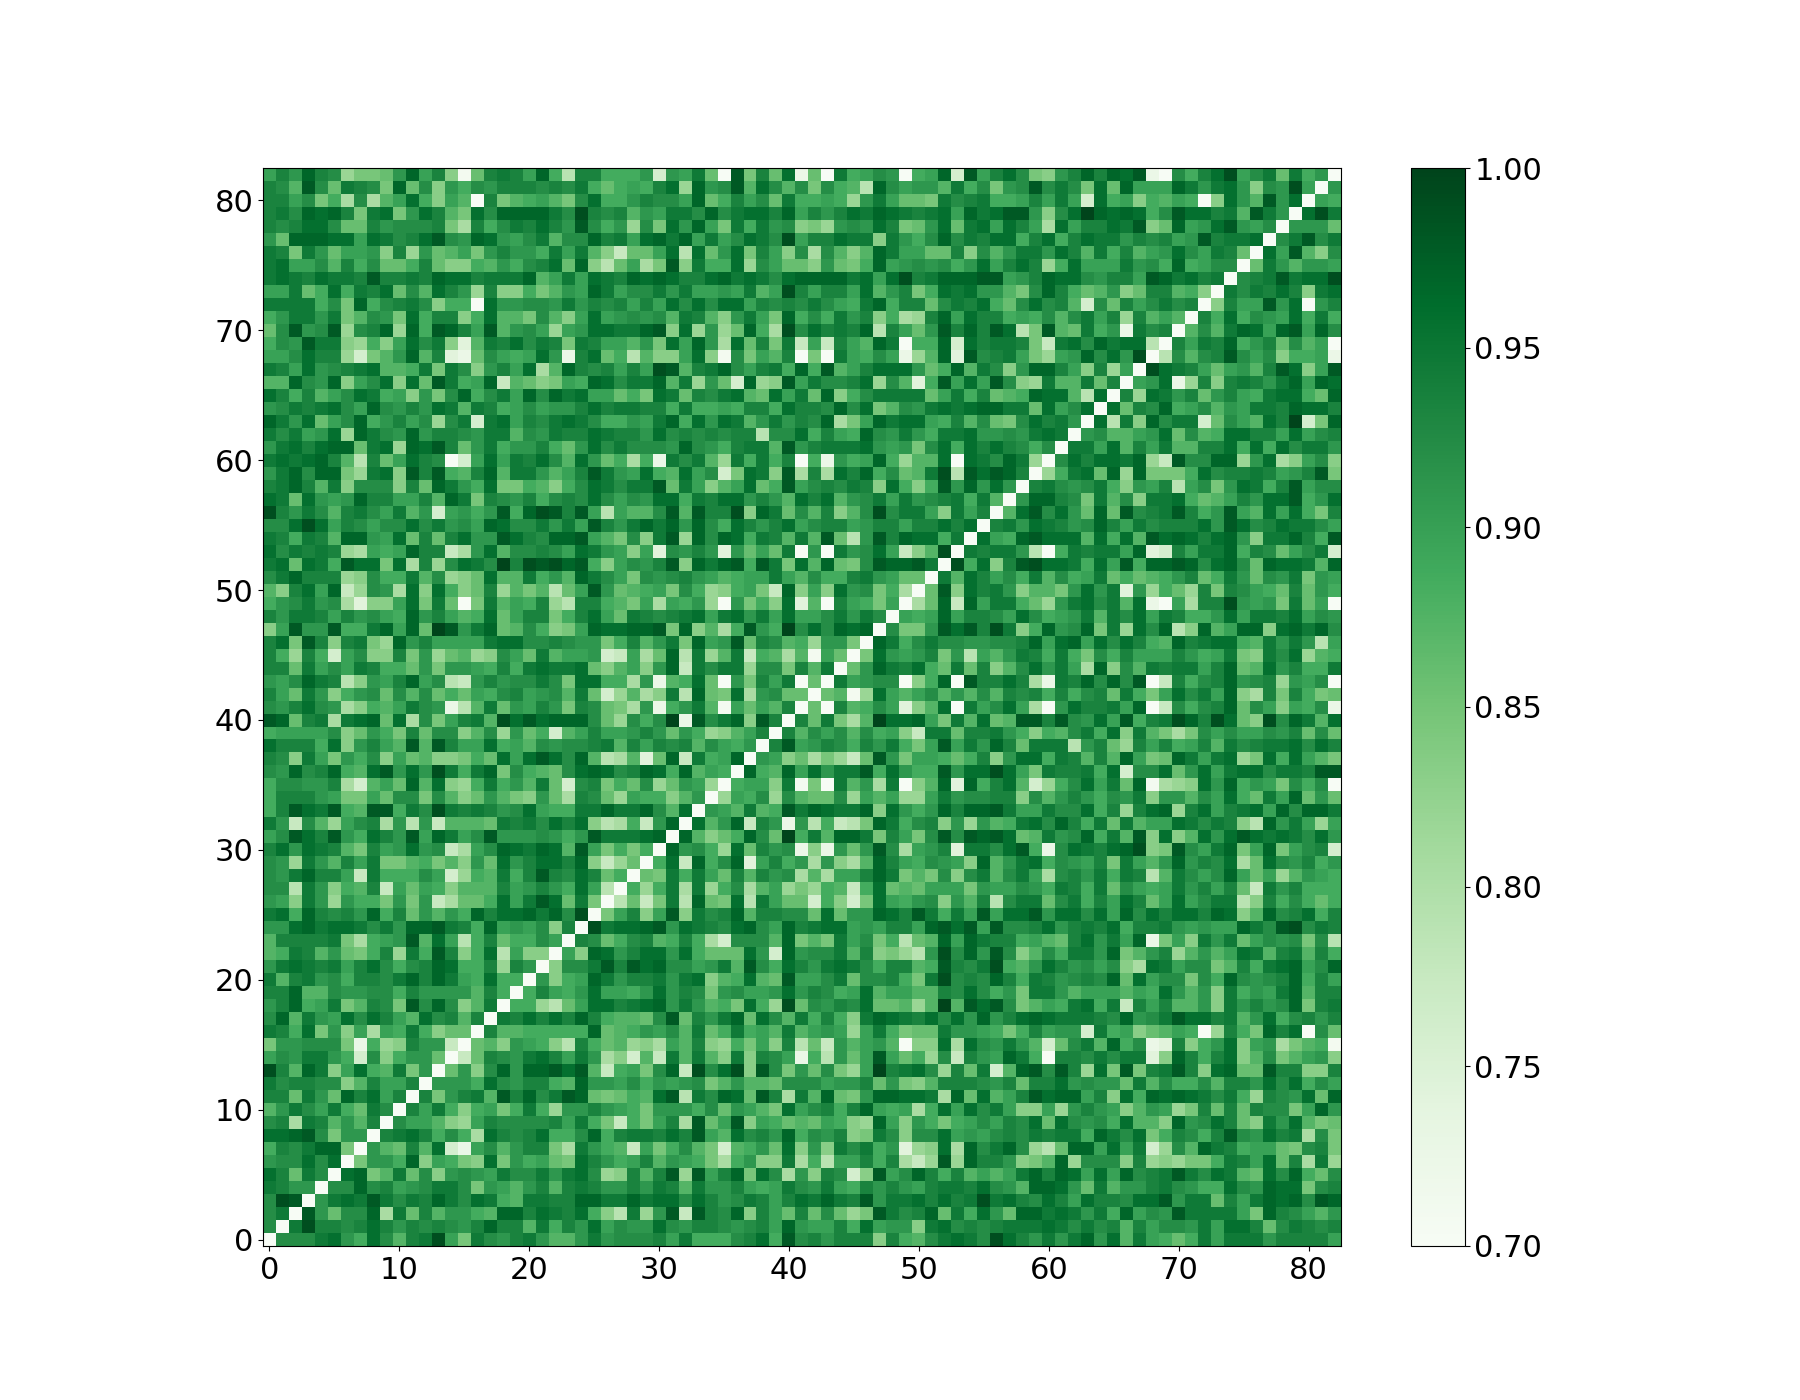
\includegraphics[width=\textwidth,height=12cm,keepaspectratio=true]{img/unigram_jaccard_50_green_07.png}
	\caption{
		Distanz zwischen den top 50 Unigrammen der Themen
	}
	\label{fig:Distanz_Unigramme}
\end{figure}

\begin{figure}[htpb]
	\centering
	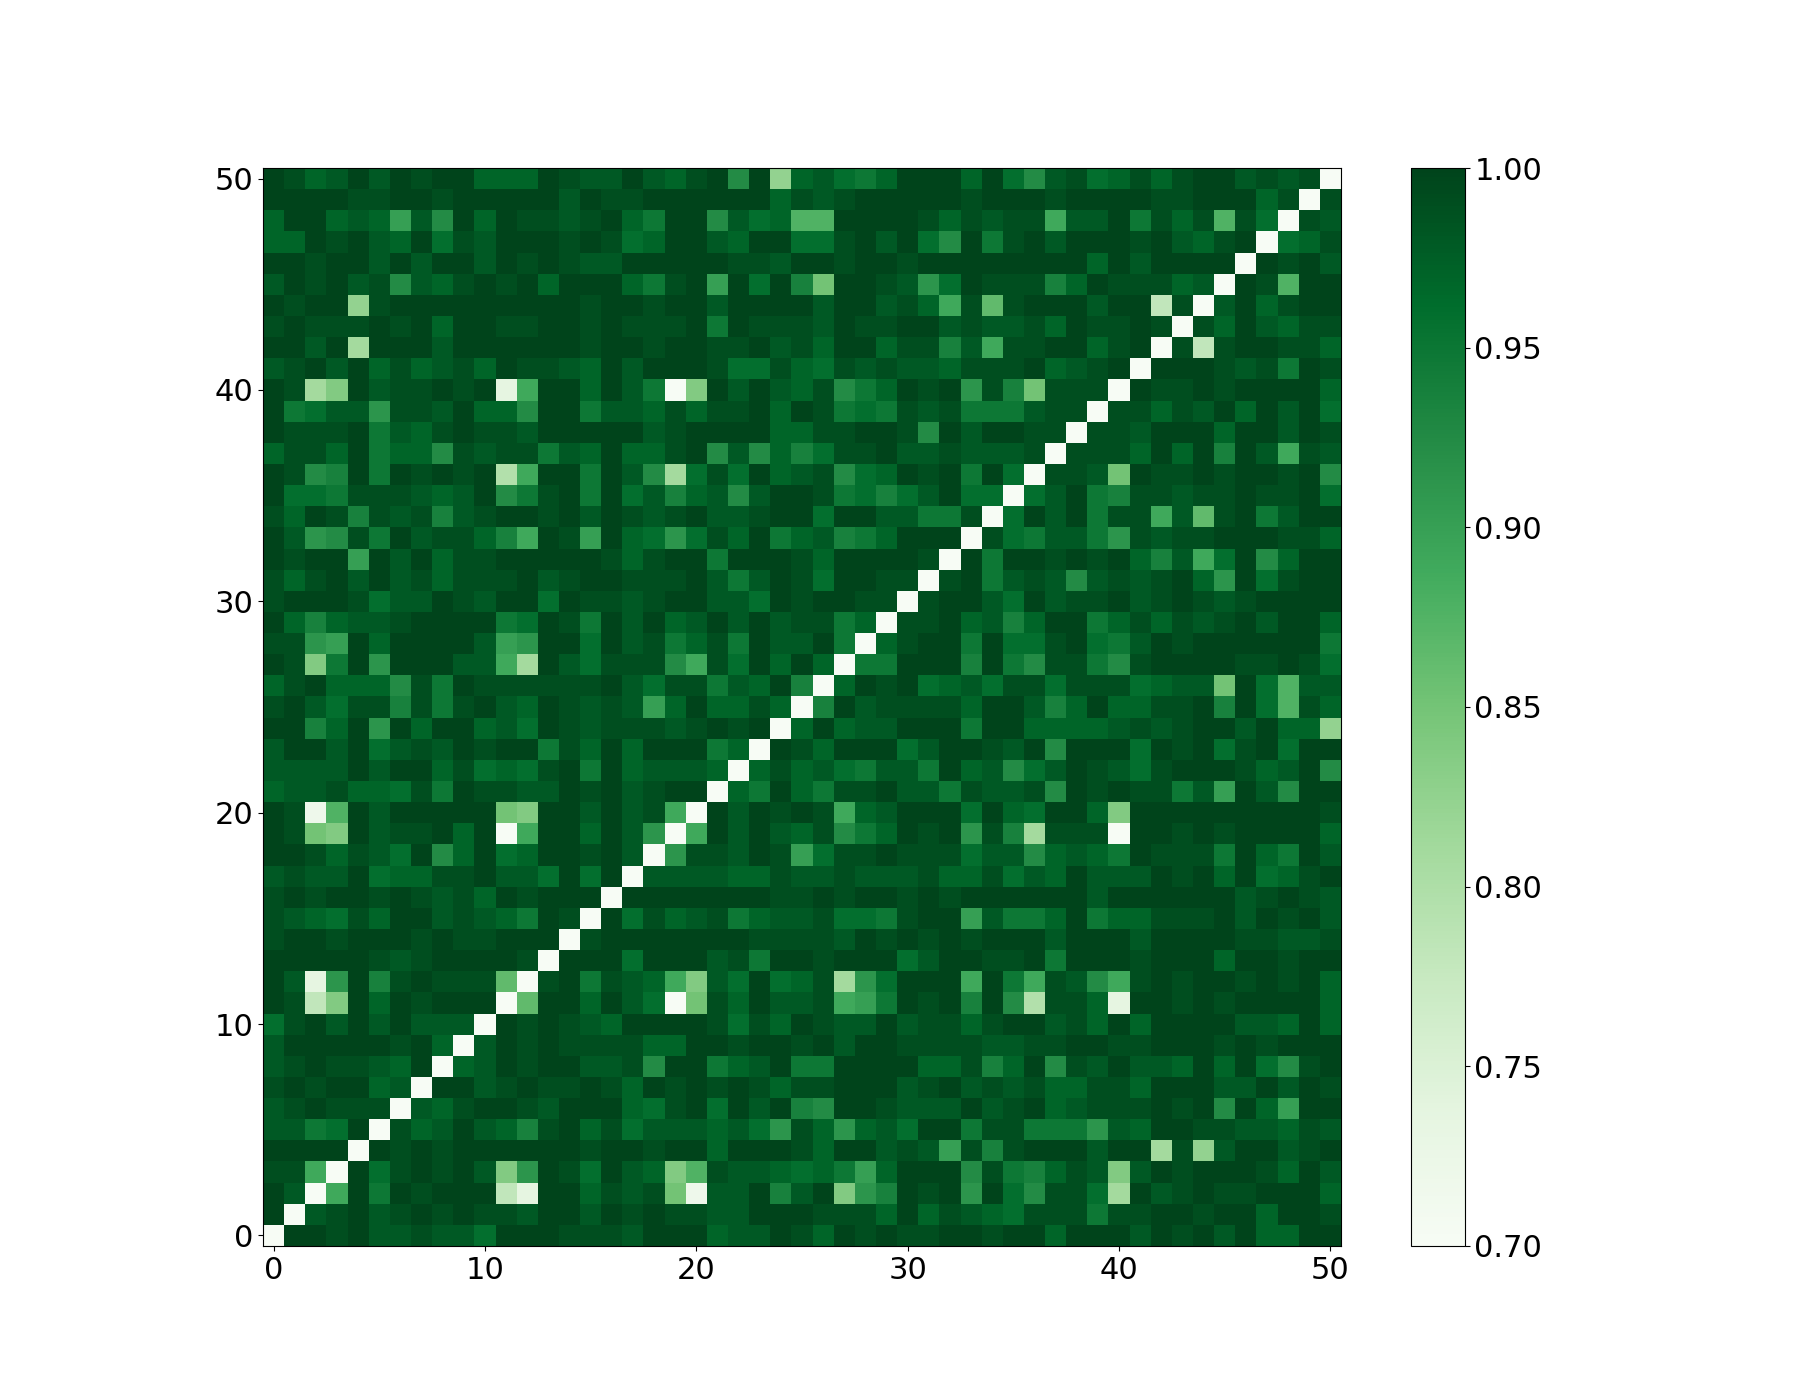
\includegraphics[width=\textwidth,height=12cm,keepaspectratio=true]{img/bigram_jaccard_50_green_07.png}
	\caption{
		Distanz zwischen den top 50 Bigrammen der Themen
	}
	\label{fig:Distanz_Bigramme}
\end{figure}
\chapter{Diskussion}

\section{}
GM-3-1-1
Topic 1 
10,066,722	63,53\%
Limited slip differentials werden mit LSD abgekürzt und daher kommen die Wörter nicht so oft vor wie sie eigentlich verwendet werden.
\chapter{Zusammenfassung und Ausblick}

\section{Zusammenfassung}


\section{Ausblick}


Es wäre gut die Trends der Cluster und Themen direkt mit \gls{dlda} zu messen und nicht nur die Trends der Terme. Die gewählten Terme beschreiben die Cluster und Themen zwar gut und grenzen sie voneinander ab aber die Trends direkt zu messen wäre eine genauere Methode.




\backmatter
\pagenumbering{roman}
\chapter{Anhang}

\begin{figure}[htpb]
	\centering
	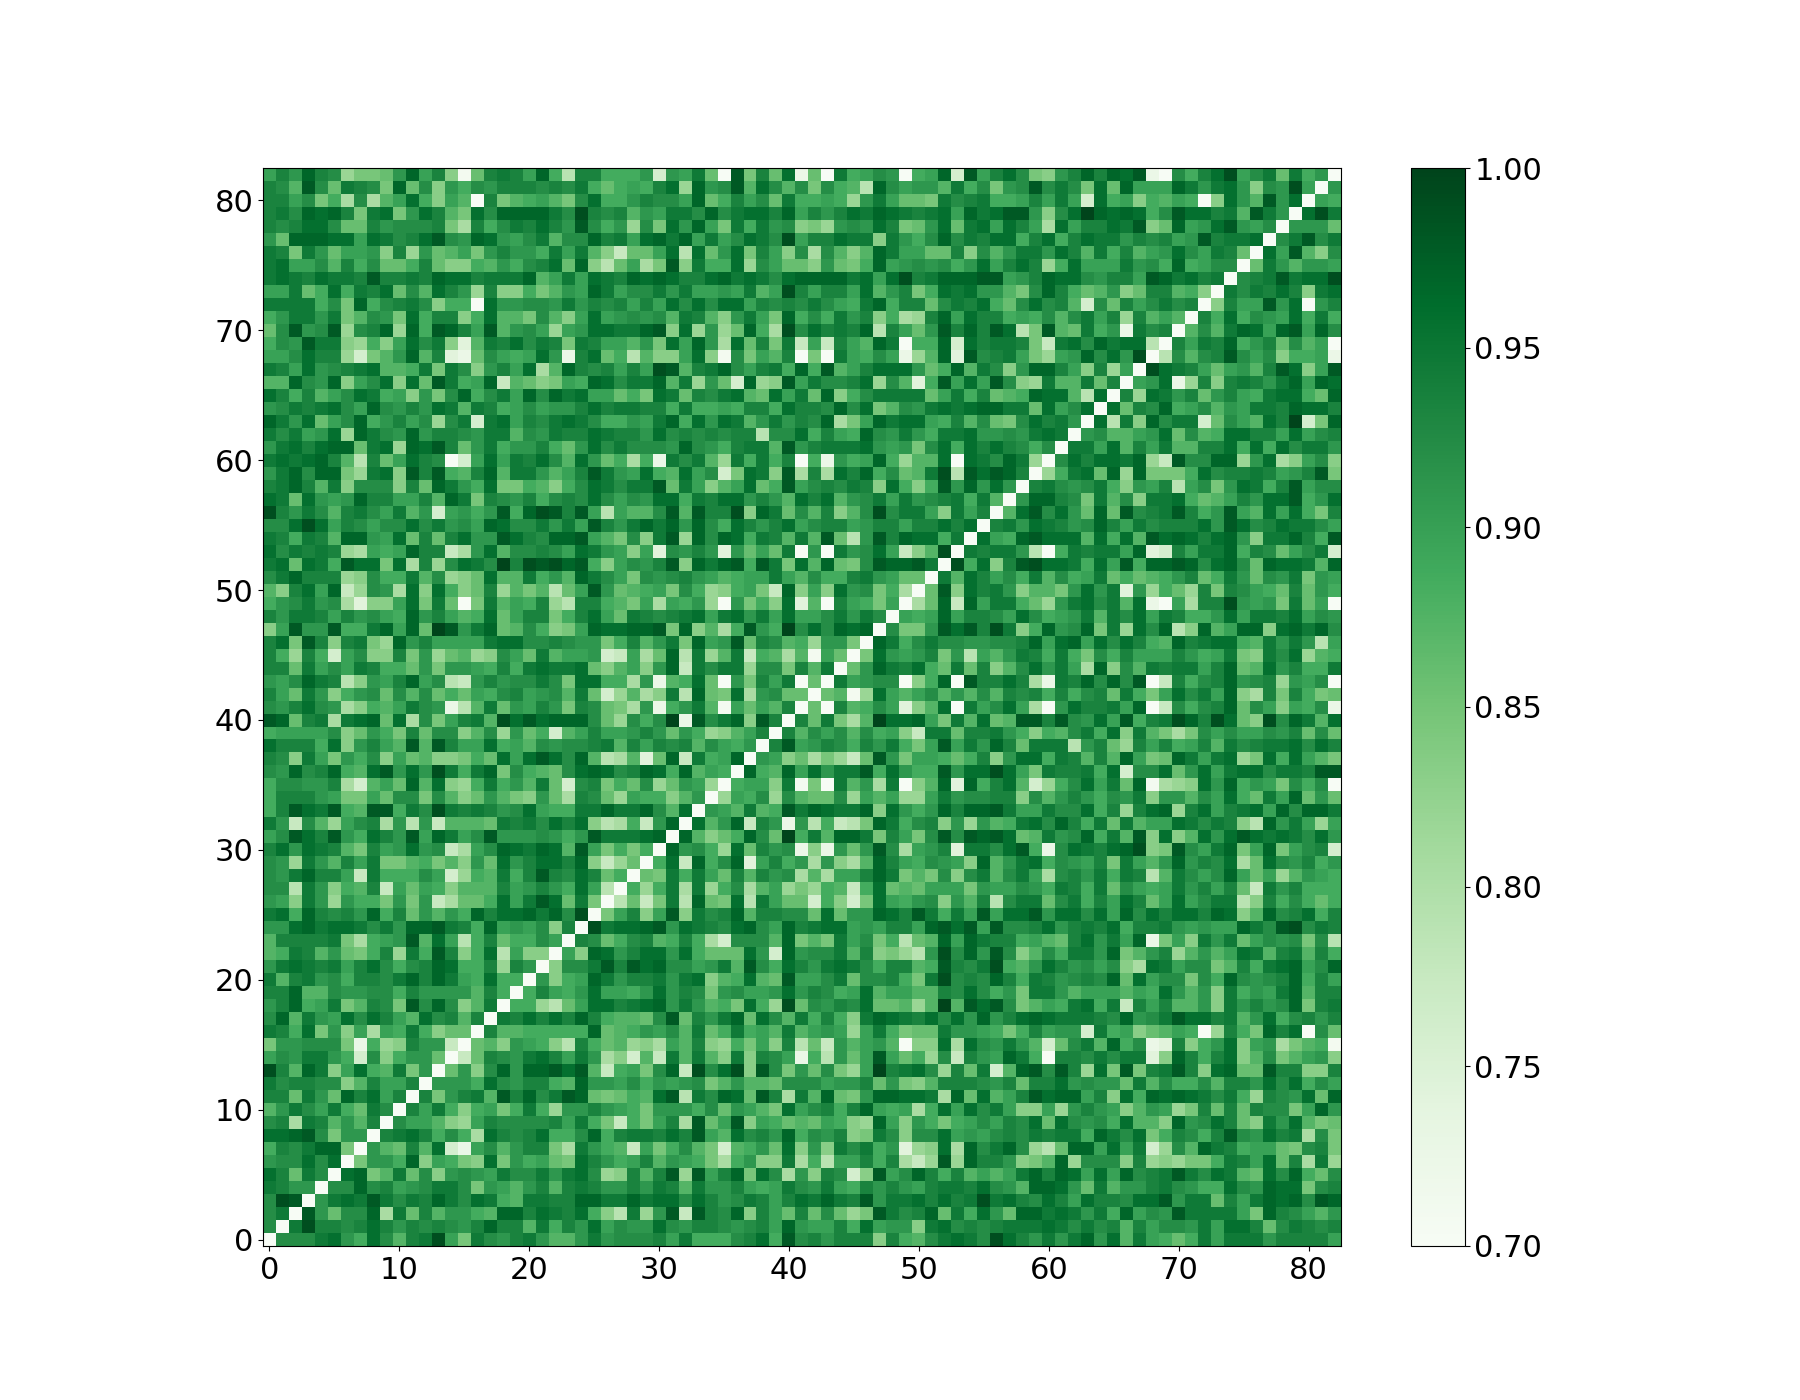
\includegraphics[width=\textwidth,height=12cm,keepaspectratio=true]{img/unigram_jaccard_50_green_07.png}
	\caption{
		Distanz zwischen den top 50 Unigrammen der Themen
	}
	\label{fig:Distanz_Unigramme}
\end{figure}

\begin{figure}[htpb]
	\centering
	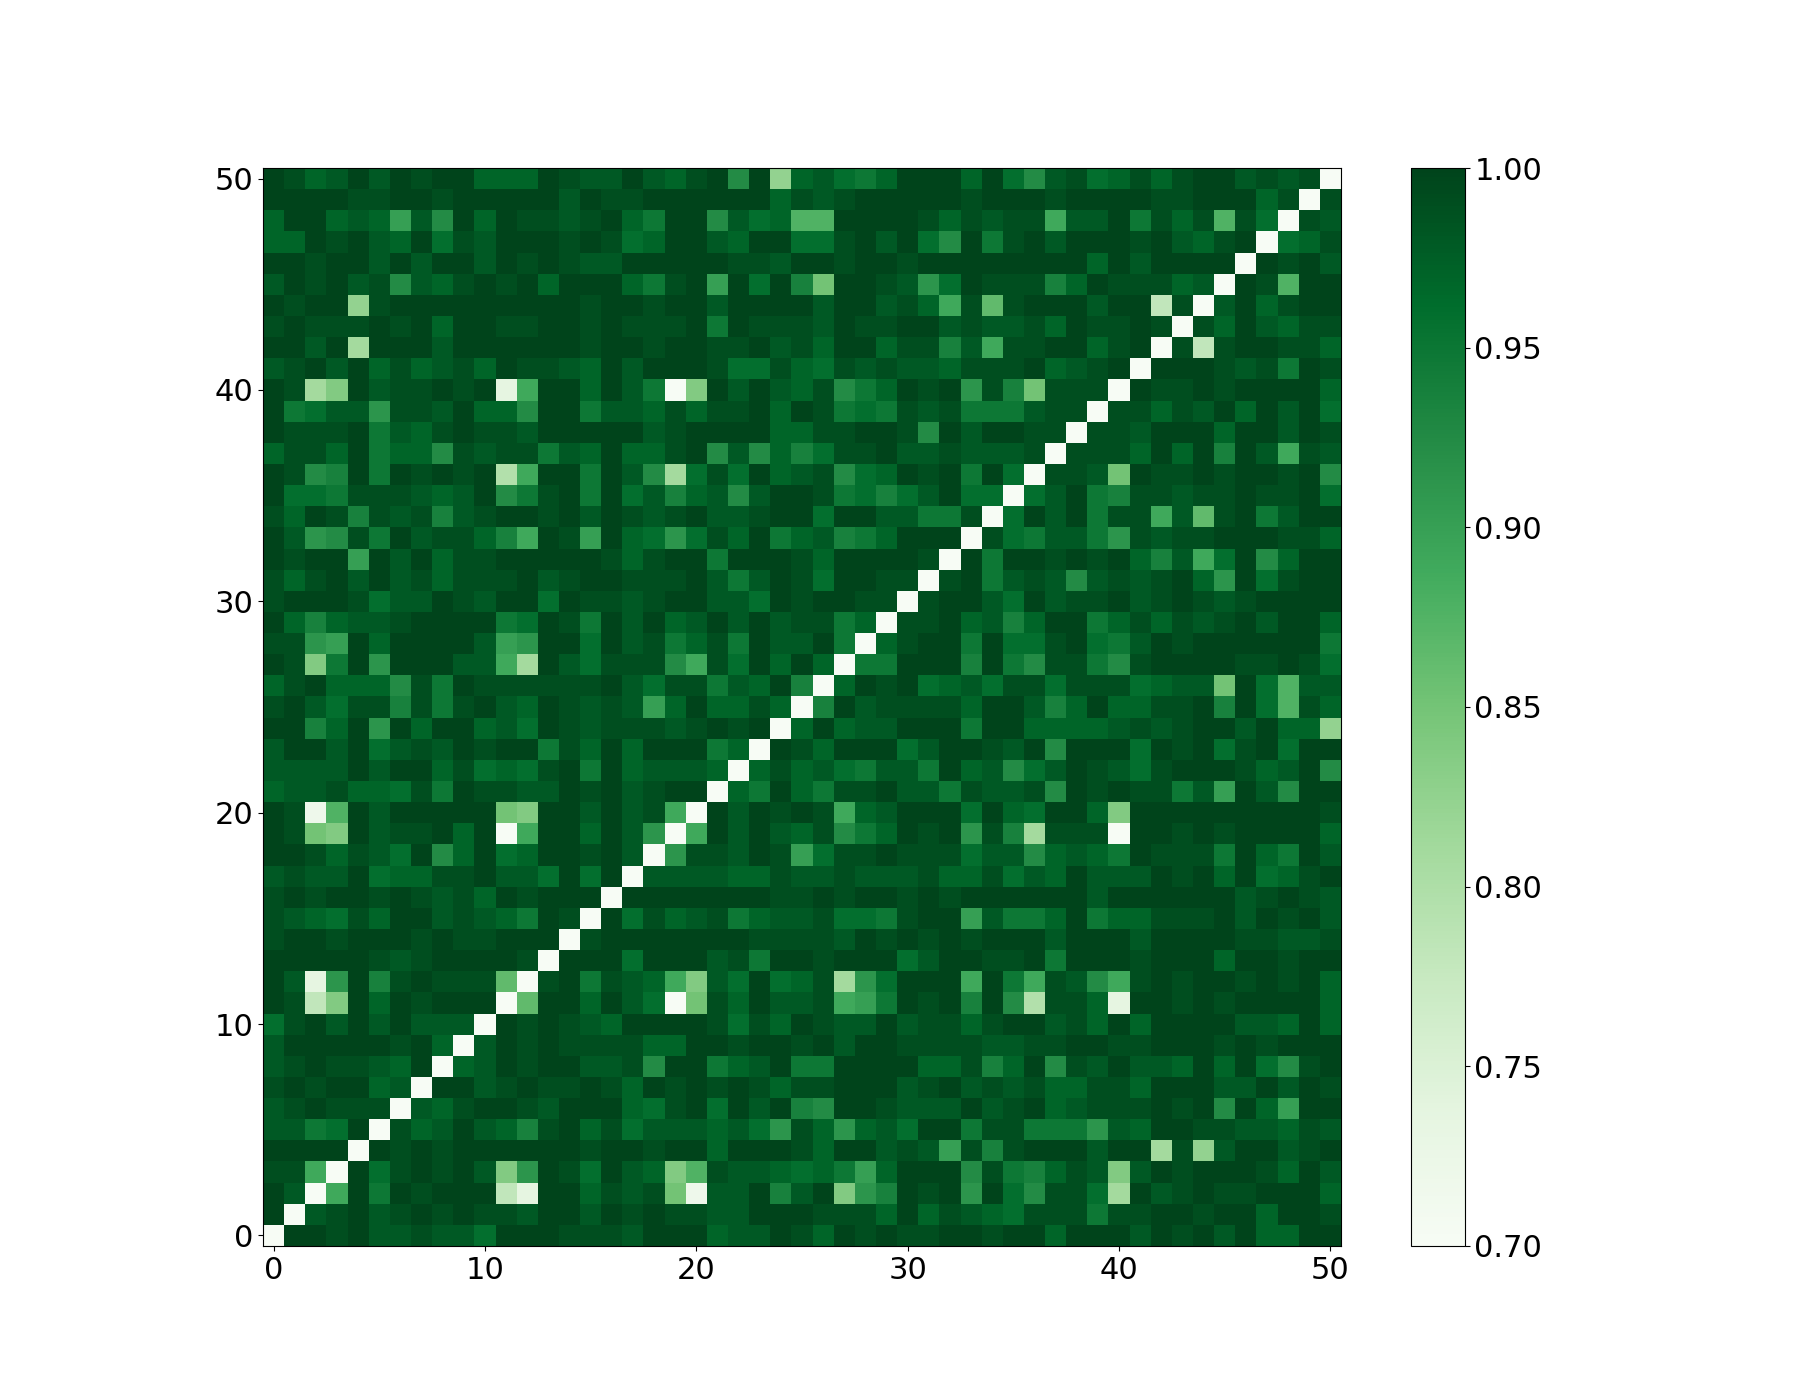
\includegraphics[width=\textwidth,height=12cm,keepaspectratio=true]{img/bigram_jaccard_50_green_07.png}
	\caption{
		Distanz zwischen den top 50 Bigrammen der Themen
	}
	\label{fig:Distanz_Bigramme}
\end{figure}
\chapter{Eidesstattliche Erklärung}
\begin{flushleft}
\Large \textbf{Erklärung zur Abschlussarbeit}
\end{flushleft}

%\normalsize

\vspace{1cm}

Ich versichere, den Bachelor-Report oder den von mir zu verantwortenden Teil einer
Gruppenarbeit*) ohne fremde Hilfe angefertigt zu haben. Ich habe keine anderen als
die angegebenen Quellen und Hilfsmittel benutzt. Alle Stellen, die wörtlich oder
sinngemäß aus Veröffentlichungen entnommen sind, sind als solche kenntlich
gemacht.

*) Bei einer Gruppenarbeit muss die individuelle Leistung deutlich abgrenzbar und
bewertbar sein und den Anforderungen entsprechen.
 
\vspace{1cm}

Bremen, den 16.11.2020

\vspace{2cm}

\begin{tabular}{@{}l@{}}\hline
	\makebox[6cm]{Hauke Tietjen}
\end{tabular}


%%%%%%%%%%%%%%%%%%%%%%%%%%%%%%%%%%%%%%%%%%%%%%%%%%%%%%%%%%%%%%%%%%%%%%%%%%%
%\no{*}
\printbibliography[heading=bibintoc,title={Literaturverzeichnis}]
%\bibliography{bibliofile}

%%%%%%%%%%%%%%%%%%%%%%%%%%%%%%%%%%%%%%%%%%%%%%%%%%%%%%%%%%%%%%%%%%%%%%%%%

\end{document}